% 
\documentclass[12pt,twoside]{report}
\usepackage{amsmath}
\usepackage{url}
\usepackage{color}
\usepackage{graphicx}
\usepackage{cite}    
\usepackage{pdflscape}
\usepackage{rotating} 
\usepackage{listings}
\DeclareGraphicsExtensions{.eps,.ps}               
\renewcommand{\vec}[1]{\mathbf{#1}}
% ====================================================================
%     Some formatting 
% ====================================================================
\topmargin -0.3in
\oddsidemargin 0.5in
\evensidemargin 0.5in
\textheight 8.5in
\textwidth 6.0in
\linespread{2}
% ====================================================================
%     The following commands tent to keep LaTex happier in the 
%     placement of figures, tables, etc
% ====================================================================
%
\renewcommand{\textfraction}{0.0}
\renewcommand{\floatpagefraction}{0.0}
\renewcommand{\topfraction}{1.0}
\renewcommand{\bottomfraction}{1.0}
\setcounter{topnumber}{9}
\setcounter{bottomnumber}{9}
\setcounter{totalnumber}{9}
% 
% ====================================================================
%     Some of the things we need for the title page
% ====================================================================
%
\author{
	\\
	by \\
	\\
      	Oleksandr Kazakov \\
	\\
        Submitted in partial fulfillment of the \\
        requirements for the degree of \\
        Doctor of Philosophy \\
        at \\
        University at Albany \\
        Department of Physics \\
        Albany, USA \\
	\\
        \\
	Advised by Professor Keith Earle and Professor Igor Lednev
	\\
	\\
}

\title{\bf{
Computational techniques in Magnetic Resonance. Applied Machine Learning for Raman Spectra Classification.}}

\date{\today}
%
%\input{definitions}
%
%%%%%%%%%%%%%% Example for content of file definitions.tex %%%%%%%%%%%
\def\ra    {\rightarrow}
\def\ul    {\underline} 
\def\mevcc {\ifmmode {\mathrm MeV}/c^2 \else MeV$/c^2$\fi}
\def\BsJpsiPhi {\ensuremath{\Bs \ra J/\psi\,\phi}}
%%%%%%%%%%%%%%%%%%%%%%%%%%%%%%%%%%%%%%%%%%%%%%%%%%%%%%%%%%%%%%%%%%%%%%
%
\begin{document} 

\thispagestyle{empty}

\maketitle

% ====================================================================
%     Generates one blank page before the 'Abstract'
% ====================================================================

\thispagestyle{empty} \cleardoublepage

% ====================================================================
% Abstract goes here
% ====================================================================
%
%\include{abstract}
%
%%%%%%%%%%%%%% Example for content of file abstract.tex %%%%%%%%%%%%%%

%%%%%%%%%%%%%%%%%%%%%%%%%%%%%%%%%%%%%%%%%%%%%%%%%%%%%%%%%%%%%%%%%%%%%%

\thispagestyle{empty} \cleardoublepage

\pagenumbering{roman}

% ====================================================================
%     Acknowledgments goes here 
% ====================================================================
%\include{acknowledgments}
%%%%%%%%%%%%%%%%%%%%%%%%%%%%%%%%%%%%%%%%%%%%%%%%%%%%%%%%%%%%%%%%%%%%%%

\tableofcontents 

\listoftables

\listoffigures

\clearpage 

\pagenumbering{arabic}

% ===================================================================
%\chapter{Introduction}
\section{Computational Sciences}
This work is built on two dissimilar research topics but in overlapping academic domains - Computational Biophysics and Analytical Chemistry. In case of Biophysics, the research work was solely based on algorithm development adapted to modern computational techniques in computer science. Specifically applied to simulate spectra for Electron Paramagnetic Resonance(Electron Spin Resonance) of nitroxide spin labels. In case of Analytical Chemistry, we performed pioneering study on application of Artificial Neural Networks compared to other advanced Machine Learning techniques for classification Alzheimer dementia on different progression stages(moderate and mild) based on Raman spectra of blood or cerebral spinal fluid.
\subsection{Electron Paramagnetic Resonance} 
Electron Paramagnetic Resonance(EPR) is a sub-branch of Nuclear Magnetic Resonance(NMR). In both NMR and EPR the interactions between electromagnetic radiation and magnetic moments are being treated. In EPR the magnetic moments arise from unpaired electrons rather then nuclei like in NMR. This spectroscopic method is widely used for investigating paramagnetic species ranging from detecting genital statistics disorders in women~\cite{2014arXiv1405.1230S} to measuring errors in single qubit rotations~\cite{2016arXiv161101110L}. Our group has a specific interest in simulating Nitroxide spin-labeled species in various motion regimes which are used as an activation site for EPR silent macromolecules providing the insights of its complex dynamics. \\ In simulating magnetic resonance spectra there are a few distinct algorithms exist which all have been developed during the mid 60's of the 20th century. Evolutionary the less computationally expensive approach have survived which is an eigenfunction expansion of density matrix~\cite{freed}. A multi‐trajectory estimation of	the spectral correlation function approach was introduced by~\cite{pedersen} and well used in our research group to model ESR Line Shape~\cite{mat_thesis}. An alternative approach~\cite{blume} that will be worked out in this thesis project is based on a master equation discretization and shares common features with modern molecular dynamics methods~\cite{sezer}. We will develop master equation discretization approach based on Blume work and describe major computational pitfalls and cost associated with it. 
\\
We will start with preparing reader for the theoretical minimum to understand the performed work. In Chapter 2 we will cover basic theory of Magnetic Resonance Spectroscopy from clasical  and statistical to quantum mechanical concepts. We will start from straight forward walk-through on phenomenological Bloch Equations describing the effect of nuclear magnetization and different relaxation mechanisms and continue with description of magnetization using density matrix approach and introducing Liouville operator.  
We will continue the discussion with the electronic $g$-tensor and hyperfine $A$-tensor anysotropies introducing their generalized forms that will be used to construct orientation dependent Hamiltonian from body to space-fixed coordinate frames where the applied magnetic field and spin operators are defined. We will also discuss distinct approach on parameterizing rotations via Euler angles or Quaternions. At the end of Chapter 2 we will describe Kubo-Anderson model\cite{kubo}\cite{anderson} of motional narrowing that was generalized by Blume which will be a fundamental for this work. In Chapter 3 we will describe developed algorithm and present the results. We will also compare number of discrete steps needed in order to completely model all spectral features.       
\subsection{Artificial Neural Network for Analytical Chemistry}

\chapter{Theoretical Background in Magnetic Resonance}
\section{Theory of Magnetic Resonance}
We discus classical and quantum mechanical theories of Magnetic Resonance and spin dynamics in this chapter. Phenomenological Bloch equations and importance of motional effects on the spectral profiles will be covered as well. We will also cover $g$ and $A$ tensors importance on the spectral line profiles and Hamiltonian transition between reference frames under the rotations. 
\subsection{Energy Splitting and Bloch Equations}
In Nuclear Magnetic Resonance(NMR) atomic nuclei or unpaired electrons in Electron Paramagnetic Resonance (EPR) in strong applied magnetic field behave like a compass needle experiencing a torque tending to align its dipole moment in the direction of the field. Macroscopically model can be studied as system of N identical distinguishable and mutually non-interacting dipoles whose population ratio can be determined in terms of Boltzmann distribution~\cite{pathria}. Each individual dipole can be well described in terms of classical mechanics as motion of gyroscope in gravitational. Precise derivation and description can of phenomena can be found in any standard classical mechanics textbook like Goldstein~\cite{gold}. Torque of such "gyroscope" can be written in terms of magnetization $\vec{M}$ and applied magnetic field $\vec{B}$:
\begin{equation}\label{eq:torque}
\vec{\tau}=\vec{M}\times\vec{B}
\end{equation}
Immediately motion of the magnetic moment can be described as following: 
\begin{equation}\label{eq:torque2}
\frac{d\vec{M}}{dt}=\gamma\vec{M}\times\vec{B}
\end{equation}
Where magnetic ratio $\gamma$ defines the ratio of a particle magnetic dipole moment to its angular momentum.\\*
On quantum mechanical level applied magnetic field creates interaction energy of the unpaired electron and it is well known as Zeeman interaction: 
\begin{equation}\label{eq:1}
E = - \vec{\mu}\cdot \vec{B}
\end{equation}  
Magnetic moment and angular momentum in terms of classical mechanics are related as: 
\begin{equation}\label{eq:2}
\vec{\mu}=\gamma \vec{J}
\end{equation}
$\vec{J}$ is related to quantum mechanical dimensionless nuclear spin operator by the form $\hbar\hat{I}$ and in terms of EPR $I$ replaced by $S$ which acts on the electron spin states rather then nuclear spin states. Taking magnetic field $B_0$ is defined along z-axis allowed energies from Eq.\ref{eq:1} can be found:
\begin{equation}\label{eq:3}
E=-\gamma\hbar S_z B_0=-\gamma\hbar m_S B_0
\end{equation} 
Where $S_z$ is a net spin of electron in $z$ direction and $m_S$ are its eigenvalues. \\*
For simple example consider nitrooxide radical that has a single unpaired electron with spin $S=1/2$ and therefore there are two possible quantum spin states $m_S=\pm1/2$. Energy displacement between higher and lower states can be calculated as:
\begin{equation}\label{eq:4}
\Delta E=\hbar \gamma B_0=\hbar \omega_0 \rightarrow \omega_0=\gamma B_0
\end{equation} 
For the picture to be more clear we can schematically represent energy level split as a diagram that is shown on Figure \ref{figure:zeeman}. It is also useful sometimes to rewrite Eq.\ref{eq:4} by introducing electronic positive $g$ factor and Bohr magneton $\mu_{\beta}$  
\begin{figure}[h!]
\begin{center}
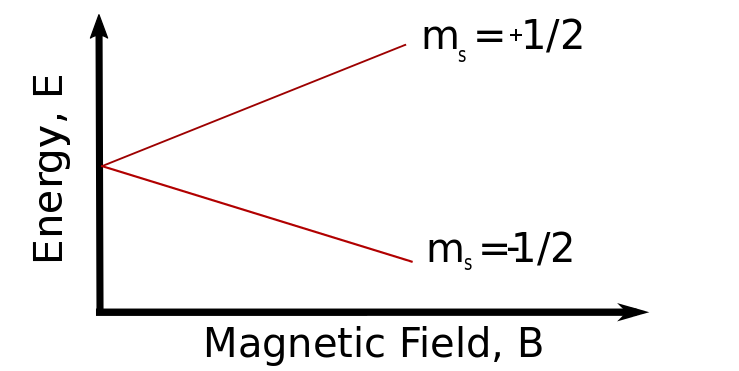
\includegraphics[width=0.7\textwidth]{figures/chap1/zems.png}
\caption{The effect of an a external magnetic field upon the energy of an electron and
the transition in induced by an a electromagnetic field for $S=\frac{1}{2}$ system in applied magnetic field $\vec B$}
\label{figure:zeeman}
\end{center}
\end{figure}
\begin{equation}\label{eq:5}
\hbar \omega_0=g\mu_{\beta}B_0 \rightarrow \omega_0=\frac{g\mu_{\beta}}{\hbar}B_0
\end{equation} 
$g$ factor carries important spectroscopic information and can be expressed as an anisotropic second rank tensor. We will cover more details on $g$ tensor in subsection 2.1.3.\\*
Meanwhile Equations \ref{eq:4} and \ref{eq:5} give a fundamental resonance condition and $\omega_0$ is known as Larmor frequency. In fact similar solution can be derived from the classical prospective as well. In 1946 Felix Bloch was the first who postulated time evolution of paramagnet "bulk" magnetization. Bloch was the first to explain magnetization of liquid samples by introducing inhomogeneity of the applied magnetic field. 
\begin{figure}[h]
\begin{center}
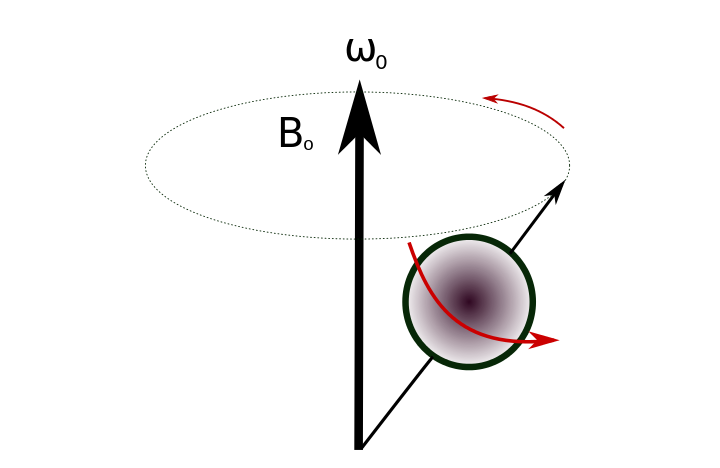
\includegraphics[scale=0.5]{figures/chap1/prec.png}
\caption{Magnetic moment precession in a constant magnetic field.}
\end{center}
\end{figure}

\begin{subequations}\label{eq:bloch}
\begin{align}
\frac{dM_x(t)}{dt}& =\gamma(M_y(t)B_z(t)-M_z(t)B_y(t))-\frac{M_x(t)}{T_2} \\
\frac{dM_y(t)}{dt}& =\gamma(M_z(t)B_x(t)-M_x(t)B_z(t))-\frac{M_y(t)}{T_2} \\
\frac{dM_z(t)}{dt} & =\gamma(M_x(t)B_y(t)-M_y(t)B_x(t))-\frac{M_z(t)-M_0}{T_1} 
\end{align}
\end{subequations}
Taking a step back to macro level. Interactions of unpaired electron spins with the environment in random and complicated fashion lead to thermal equilibrium defined by Boltzmann factor. In other words if number of nuclear or electron spins pointing up or down defined as $N_{\uparrow}$ and $N_{\downarrow}$ population ratio defined as follows:
\begin{equation}\label{eq:8}
\frac{N_{\downarrow}}{N_{\uparrow}}=exp(-\Delta E/k_{b}T)
\end{equation}
Where $k_b$ is a Boltzmann constant and $T$ is a sample temperature. This interactions lead to known as spin-lattice relaxation mechanism defined by longitudinal relaxation time $T_1$. 
On other hand various interactions between spins will not directly affect population ratio but will tend to cause transverse magnetization to decay and mechanism is known as spin-spin relaxation and characterized by time constant $T_{2}$. \\*
Effective magnetic field $B_{eff}$ due to preceding inhomogeneity can be written as following:
\begin{equation}\label{eq:inhomog2}
B_{eff}=B_0+B_1(t)
\end{equation}
Additional time-dependent field is added. In order to eliminate time dependence in fluctuating magnetic fields appropriate coordinate system should be chosen. In the rotating frame fixed static field has an additional term of $\frac{\omega_0}{\gamma}$ thus in the rotating frame
\begin{equation}\label{eq:inhomog}
B_{eff}=(B_0+\frac{\omega_0}{\gamma})\vec{i}+B_1\vec{j}
\end{equation}
As example construction of Bloch equations for low $B_1$ to avoid saturation effects can be easily shown. Choosing unit vector $i$ to be in parallel with $z(\hat{z})$ and direction of oscillating field in laboratory frame defined in $x$ direction($\hat{x}$)  and define 
 \begin{equation}\label{eq:inhomog3}
B_1=-\frac{\omega_1}{\gamma}2\cos\omega t\hat{x}
\end{equation}
In the rotating frame Bloch equations from \eqref{eq:bloch} can be rewritten as: 
\begin{subequations}\label{eq:bloch2}
\begin{align}
\frac{dM_x(t)}{dt}& =\Delta\omega M_y-\frac{M_x(t)}{T_2} \\
\frac{dM_y(t)}{dt}& =-\Delta\omega M_x-\frac{M_y(t)}{T_2}-\omega_1M_z \\
\frac{dM_z(t)}{dt} & =\omega_1M_y-\frac{M_z(t)-M_0}{T_1} 
\end{align}
\end{subequations}
Difference between Larmour and irradiation frequencies gives the energy absorption in the system and defined as $\Delta\omega=\omega-\omega_0$ and conditionally it defines resonance phenomenon. Evolution of net magnetization of the sample can be generalized and predicted in terms of Bloch equations solving it with the specific to the system constraints. For high field experiments when $B_0 \sim B_1$ or including line saturation, harmonic generation, multiquantum transitions and etc. solution becomes not trivial. 
\subsection{Density Matrix} 
Magnetization quantum mechanically can be found as expectation value of quantum operators like nuclear or spin angular momentum ones. Technique to treat time evolution of the magnetization is given through the density matrix approach.\\* 
Lets Assume that wave function is a product of two wave functions: 
\begin{equation}\label{eq:10}
|\psi_{total}\rangle=|\psi_{system}\rangle|\psi_{enviroment}\rangle=\sum_{i,j} c_{i,j}|\psi_{i(system)}\rangle|\psi_{j(enviroment)}\rangle
\end{equation}
The expectation value of an observable that operates only on the system($S,I$ spin operators) can be written in complete set of basis states as:
\begin{equation}\label{eq:11}
\langle A \rangle=\sum_{i,j} c_{i,j}^*c_{k,l}^*\langle \theta_{(j(env))}|\langle \phi _{i(sys)}|A|\phi_{k(sys)}\rangle|\theta_{l(env)}\rangle=\sum_{i,k}\rho_{k,i}A_{i,k}
\end{equation}
Where $\rho$ is known as density matrix and and coefficients $c_{i,j}$ modeling a coupling  provides useful and powerful way to characterize the state of the ensemble of quantum system. 
Density matrix is hermitian thus it can be diagonalized and written as following: 
\begin{equation}\label{eq:13}
\hat{\rho}=\sum_{ij}\rho_{ij}|\phi_i\rangle\langle \phi_j|
\end{equation} 
Where $\rho_{ij}$ are eigenvalues. 
Using Schroedinger equation one can find: 
\begin{equation}\label{eq:14}
\frac{\partial \hat{\rho}}{\partial t}=\frac{1}{i\hbar}\sum_{ij}\rho_{ij}\Big[\Big(\frac{\partial}{\partial t}|\phi_i\rangle\Big)\langle \phi_j|+|\phi_i\rangle\ \Big[\Big(\frac{\partial}{\partial t}\langle \phi_j|\Big)\Big]
\end{equation} 
Or recalling Schroedinger Equation from childhood memories can be rewritten as: 
 \begin{equation}\label{eq:15}
\frac{\partial \hat{\rho}}{\partial t}=\frac{1}{i\hbar}[\hat{H},\hat{\rho}]
\end{equation} 
In such motion observables are time independent and density operator is time-dependent. 
This equation can be directly solved in vector space known as Liouville where $\rho$ can be represented as vector. Eq.\ref{eq:15} can be rewritten as:
 \begin{equation}\label{eq:16}
\frac{d\rho_{ij}}{dt}=\frac{1}{i\hbar}\sum_{k,l}(H_{ik}\delta_{lj}-\delta_{ik}H_{jl}^T)\rho_{kl}=-\frac{i}{\hbar}\sum_{k,l}\mathcal{L}_{ij,kl}\rho_{kl}
\end{equation} 
Where $\mathcal{L}$ defines the Liouville super-operator which operates on Hilbert space operators. In this notation each matrix element is labeled by two indexes. Such unusual notation will later bring a computational simplification for Magnetic Resonance computations. 
using Kroenecker tensor product super-operator can be written as 
\begin{equation}\label{eq:17}
\hat{\mathcal{L}}=\hat{H}\otimes\hat{I}-\hat{I}\otimes\hat{H}^{T}
\end{equation} 
Where $\hat{I}$ is a unit matrix of rank of $\hat{H}$
As simple example for nuclei or spin 1/2 operator time-dependent Hamiltonian can be written as: 
\begin{equation}\label{eq:18}
\hat{H} = \begin{bmatrix}
       0 & f^*           \\[0.3em]
       f & 0 \\[0.3em]
     \end{bmatrix}
\end{equation}
Liouville supermatrix is following: 
\begin{equation}\label{eq:19}
\hat{\mathcal{L}} = \begin{bmatrix}
       0 & -f & f^* & 0          \\[0.3em]
       -f^* & 0 & 0 & f^* \\[0.3em]
       f & 0 & 0 & -f \\[0.3em]
       0 & f & -f^* & 0 
     \end{bmatrix}
\end{equation}
The ordering of the rows and columns of $\hat{\mathcal{L}}$ are all equivalent up to a unitary transformation, but the ordering of the rows and columns of $\hat{\mathcal{L}}$ arising from the definition of the Kronecker tensor product is perhaps the easiest to follow. As example, the $\hat{\mathcal{L}_{1/2,1/2;-1/2,1/2}}$ matrix element arises from $\hat{\mathcal{H}_{1/2,-1/2;}\delta_{1/2,1/2}}=f^*$. Another example that is  for calculation is spin 1 system. Assuming that Hamiltonian give as: 
\begin{equation}\label{eq:hamliv}
\hat{\mathcal{H}} = \begin{bmatrix}
       g & f^* & 0 \\[0.3em]
       f & 0 & f^* \\[0.3em]
       0 & f & -g \\[0.3em]
     \end{bmatrix}
\end{equation}
Corresponding Liouville matrix has a following form: 
\begin{equation}\label{spinoneliv}
\hat{\mathcal{L}} = \begin{bmatrix}
       0 & -f & 0 & f^* &0 & 0 & 0 & 0 & 0         \\[0.3em]
       -f* & g  & -f   & 0 &f^* & 0  & 0   & 0 & 0         \\[0.3em]
       0 & -f^*  & 2g   & 0 &0 & f^*  & 0   & 0 & 0         \\[0.3em]
       f & 0  & 0   & -g &-f & 0  & f^*   & 0 & 0         \\[0.3em]
       0 & f  & 0   & -f^* &0 & -f  & 0   & f^* & 0         \\[0.3em]
       0 & 0  & f   & 0 &-f^* & g  & 0   & 0 & f^*         \\[0.3em]
       0 & 0  & 0   & f &0 & 0  & -2g   & -f & 0         \\[0.3em]
       0 & 0  & 0   & 0 &f & 0  & -f^*   & -g & f-         \\[0.3em]
       0 & 0  & 0   & 0 &0 & f  & 0   & -f^* & 0         \\[0.3em]
     \end{bmatrix}
\end{equation}
There are different approaches on algorithm of Liouville matrix construction that can be useful if number $S>1$ and construction by hand can lead to difficultly traceable error.In more details  discussed in Gamilel~\cite{gam}.   
\subsection{The g-tensor}
In crystaline and liquid systems EPR spectra may dependent on orientation of the sample relative to applied magnetic field $B_0$ this also known as spectrum anistopy. Consider Zeeman term for spin Hamiltonian given as: 
\begin{equation}\label{eq:20}
\mathcal{\hat{H}}=\beta \vec{B}\cdot g \cdot \hat{S}
\end{equation} 
In Eq.\ref{eq:20} $g$ factor is represented as 2-nd rank tensor. Anisotropy of the $g$ factor arises from spin-orbit coupling between the ground state and excited states. If applied magnetic field is chosen in the direction of cosines$(\hat{i},\hat{j},\hat{k})$ in the laboratory frame with $S_z$ to be diagonal a simple example is to construct Hamiltonian matrix and define its eigenvalues for $S=1/2$:

\begin{equation}\label{eq:21}
\mathcal{H} = \begin{bmatrix}
       \frac{1}{2}\beta B_0( \hat{i}g_{xz}+\hat{j}g_{yz}+\hat{k}g_{zz}) & \frac{1}{2}\beta B_0( \hat{i}g_{xx}+\hat{j}g_{xy}+\hat{k}g_{xz})          \\[0.3em]
  & -i(\hat{i}g_{xy}+\hat{j}g_{yy}+\hat{k}g_{yz}) \\[0.3em]      
       \frac{1}{2}\beta B_0( ig_{xx}+jg_{xy}+kg_{xz})  &  -\frac{1}{2}\beta B_0( \hat{i}g_{xz}+\hat{j}g_{yz}+\hat{k}g_{zz}) \\[0.3em]
        -i(\hat{i}g_{xy}+\hat{j}g_{yy}+\hat{k}g_{yz})  & \\[0.3em]
     \end{bmatrix}
\end{equation}
Values of the $g$ factor matrix can be found from difference between eigenvalues of the Hamiltonian matrix in Eq.\ref{eq:21}. General form is given as: 

\begin{equation}\label{eq:gtengeneral}
\begin{array} {lcl} &g^2& = g_{xx}^2\sin^2\theta\cos^2\phi+2g_{xy}^2\sin^2\theta cos\theta+g_{yy}^2sin^2\theta\\ & + & g_{yy}\sin^2\theta\sin^2\phi+2g_{xz}\cos\theta\sin\theta\cos\phi\\ & + & 2g_{yz}\cos\theta\sin\theta\sin\phi+g_{zz}\cos^2\theta \end{array}
\end{equation}
Matrix elements can be determined experimentally by the finite number of rotations of the sample or applied magnetic field in $xy,yz$ and $xz$ planes. For $xz$ plane $\theta$ is an angle between magnetic field and $z$ axis and $\phi=0$ $g$ teson has a following form:  
\begin{equation}\label{eq:22}
g^2=g_{xx}^2\sin^2\theta+2g_{xz}^2\sin^2\theta \cos\theta+g_{zz}^2\cos^2\theta
\end{equation} 
When $yz$ plane is rotated around $\phi=90^{\circ}$:
\begin{equation}\label{eq:newone22}
g^2=g_{yy}^2\sin^2\theta+2g_{yz}^2\sin\theta cos\phi+g_{zz}^2sin^2\theta\cos\phi\sin\phi
\end{equation} 
And finally for the $xy$ plane $\theta=90^{\circ}$:
\begin{equation}\label{eq:newone221}
g^2=g_{xx}^2cos^2\phi+2g_{xy}^2\sin\phi\cos\phi+g_{yy}^2\sin^2\phi
\end{equation} 
In order to obtain unique values of the $g$ tensor three measurements in each plane will be suitable. For example if $\theta=0$ and $\theta=90^{\circ}$ one can obtain $g^2_{xx}$ and $g^2_{zz}$. Matrix $g^2$ can be diagonalized by casting direction of cosines which define molecular frame to laboratory frame. Hamiltonian in principal axis of $g$ tensor can be written as: 
\begin{equation}\label{eq:princham}
\mathcal{H}=\vec{B}\cdot \begin{bmatrix} g_{xx} & 0 & 0 \\ 0 & g_{yy} & 0\\ 0 & 0 & g_{zz}\end{bmatrix}\cdot \hat{S}
\end{equation}   
Thus matrix calculation reduced from finding nine elements to three which is enough to obtain important geometrical and quantum mechanical information on a species.For symmetric magnetic samples axis coincide with principal axis of $g$ tensor and symmetry planes are usually perpendicular to them. For molecules like eclipsed ethane with low symmetry the principal axes orthogonal to each other can point to arbitrary direction specified by local magnetic field. \\*
There are in general three groups of symmetry: cubic, uniaxial and rhombic and presented of Fig.\ref{figure:gsym}. For the cubic symmetry principal values of $g$ tensor are equal to each other $g_{xx}=g_{yy}=g_{zz}$ so that anisotropy in EPR spectra vanishes and absorpion spectrum presented as one Lorentzian lineFig.\ref{figure:gsym}(a). Uniaxial case when $g_{xx}=g_{yy}<g_{zz}$ or $g_{xx}=g_{yy}>g_{zz}$ shape of the absorption and derivative spectrum has a step sides Fig.\ref{figure:gsym}(b),(c). Rhombic symmetry Fig.\ref{figure:gsym}(d) is given when $g_{xx}\neq g_{yy}\neq g_{zz}$ and typical for nitrooxides that are of interest for our group. 
\begin{figure}[h!]
\begin{center}
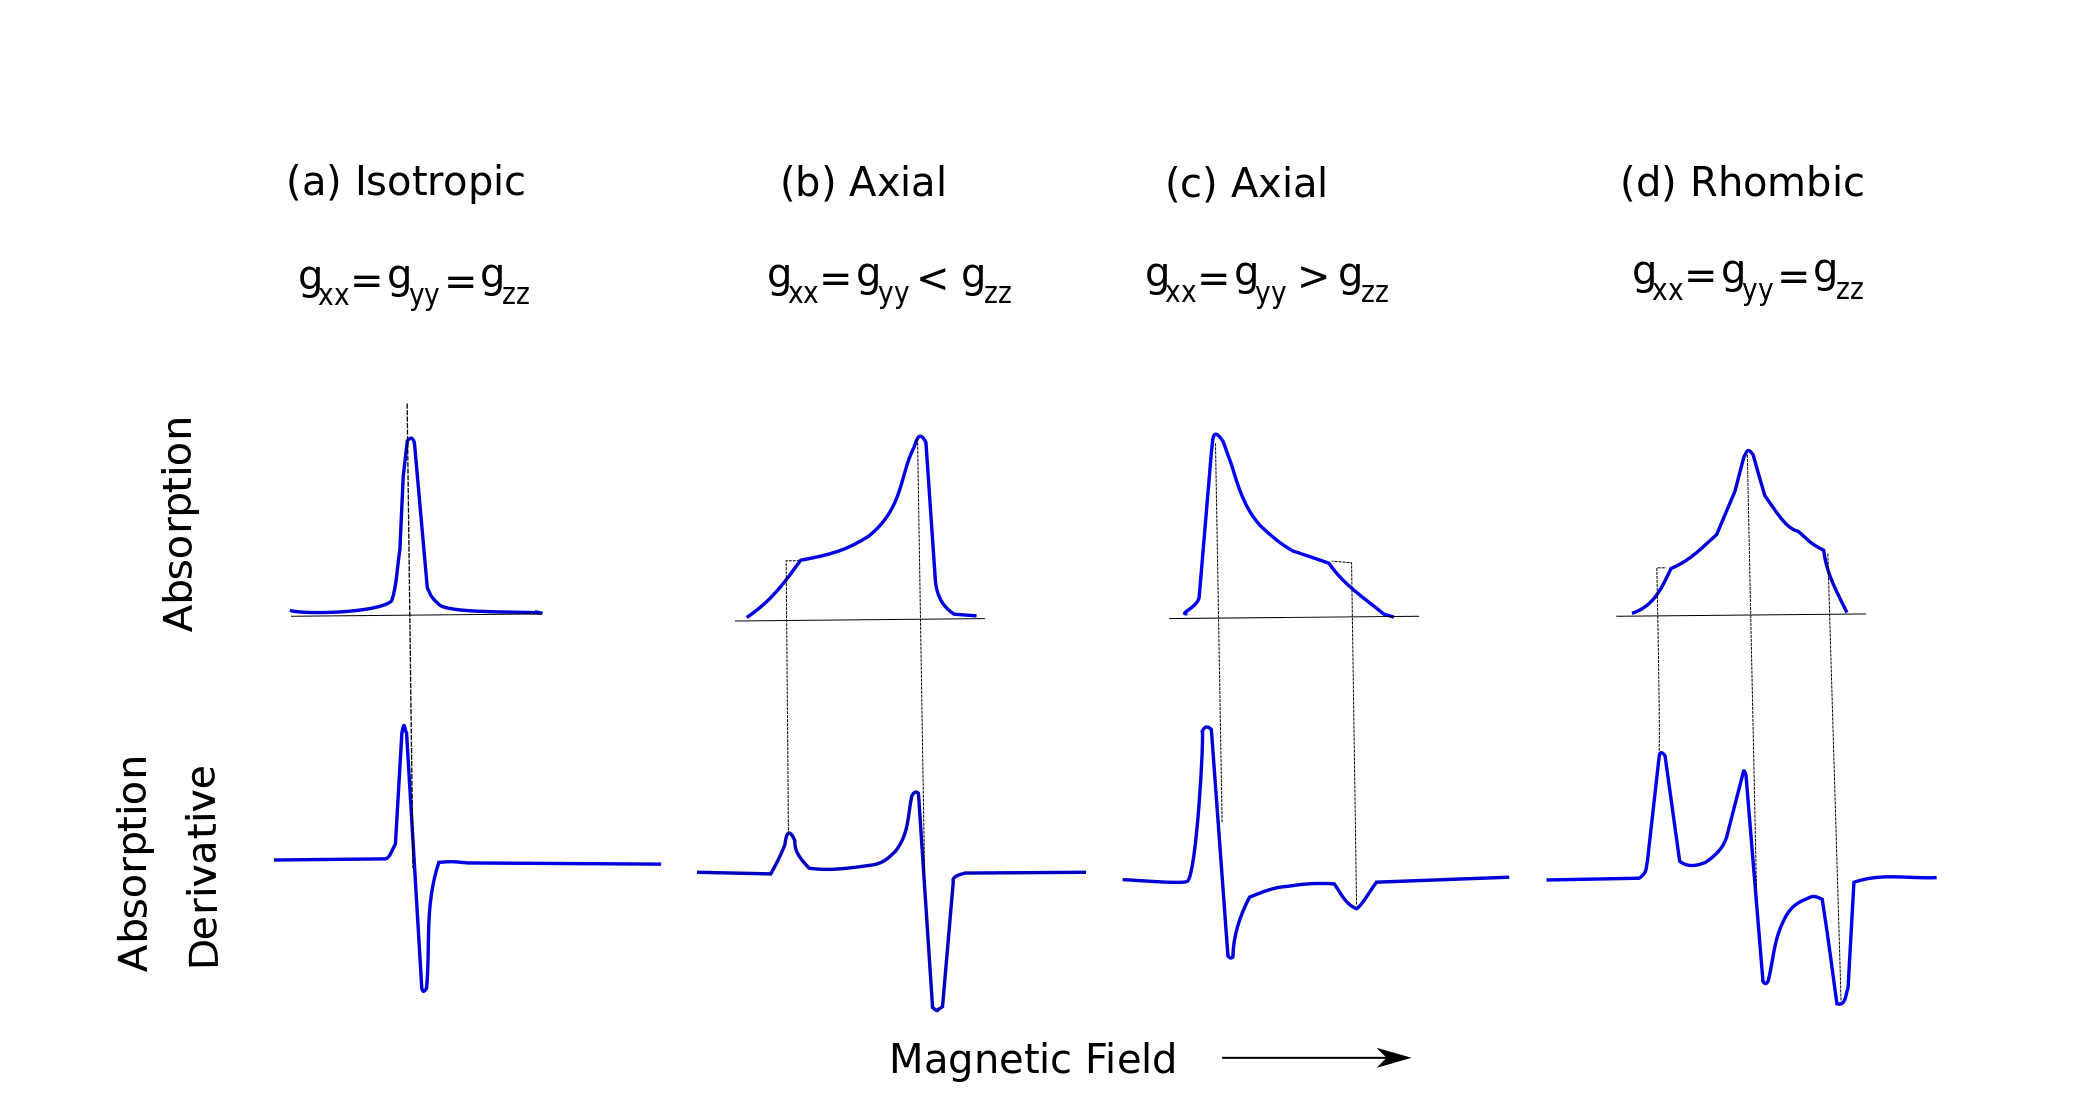
\includegraphics[width=1\textwidth]{figures/chap1/gten1.png}
\caption{Absorpton lineshape and its derrivative for randomly oriented spin system with (a) cubic(isotropic) symmetry; (b),(c) uniaxial symmetry and (d) rhombic symmetry.}
\label{figure:gsym}
\end{center}
\end{figure}
\\*
If to go $\hbar$-deeper deviations from electron $g_e$ arise from spin-orbit coupling.  $g$ tensor may be written as:
\begin{equation}\label{eq:gtenelec}
\pmb{g}=g_e\hat1+\Delta \pmb{g}_{SO/OZ}+\Delta\pmb{g}_{RMC}+\Delta\pmb{g}_{GC}
\end{equation} 
First term is a free electron $g$-factor and its value $g_e=2.0023...$ multiplied by the identity matrix. Second term represents spin orbital/orbital-Zeeman coupling, second term is known as "mass-velocity" correction and third term is a gauge correction they are both diamagnetic and much smaller compared to the first term. In order to find spin-orbit/orbial-Zeeman term from second order perturbation theory excited states $|n\rangle$ and ground states $|0\rangle$ should be determined for quantum mechanical system. Shift can be written as~\cite{thesis1}:  
\begin{equation}\label{eq:zeemanparamagn}
\Delta \pmb{g}_{SO/OZ}=\frac{2g_e\beta_e^3}{\hbar^2k_0c^2\langle S_z\rangle}\sum_N Z_N\sum_n\Bigg[ \frac{\langle0|\hat{\pmb{O}_1}|n\rangle\langle n|\hat{\pmb{O}_2}|0\rangle}{E_0^{(0)}-E_n^{(0)}}+c.c\Bigg]
\end{equation} 
Here $N$ is order of nuclei and $"c.c"$ are complex conjugate of spin-orbit coupling integrals.For 1-electron coupling integral is given as:
\begin{equation}\label{eq:oneel}
\langle 0|\sum_i\frac{1}{r^3_{iN}}\times(\hat1_{iN})_us_{iz}|n\rangle\langle n|\sum_j(\hat1_{iN})_v|0\rangle
\end{equation}
And integral for 2-electron coupling can be written as:
\begin{equation}\label{eq:oneel}
\langle 0|\sum_{ij}[\pmb{r}_{ij}\times(\nabla_i-2\nabla_j)]_us_{jz}|n\rangle\langle n|\sum_j(\pmb{r}_k\times\nabla_k)_v|0\rangle
\end{equation}
Where summation is done over all orbitals $(i,j)$ and $u,v$ are the Cartesian axises.
\subsection{A-tensor}
The interaction between spin of unpaired electron with local magnetic fields which are product of spin of nuclei in the molecule where electron is located can lead to additional spectral lines. Electron and nuclear spins are quantized thus number of lines for a single nuclei can be found as $2I+1$ and they are clustered around major Zeeman energy levels. This interaction is known as Nuclear Hyperfine interaction. Separation between this additional lines determined by the hyperfine coupling constant. Hamiltonian for hyperfine interaction can be written~\cite{nordio}: 
\begin{equation}\label{eq:23}
\mathcal{\hat{H}}_{hf}=-g_e\beta_eg_N\beta_N\Big[\frac{(\hat{I}\cdot \hat{S})r^2-3(\hat{I}\cdot\vec{r})(\hat{S}\cdot\vec{r})}{r^5}-\frac{8\pi}{3}(\hat{I}\cdot\hat{S})\delta(\vec{r})\Big]
\end{equation} 
Where $\vec{r}$ is a electron-nucleus distance, $g_N$ and $\beta_N$ are nucleus g factor and Bohr magneton respectively. First term represents dipolar coupling of electron to nucleus~\cite{car} and can be derived from interaction energy between an electron and nucleus that are located distance $r$ from each other so that quantum mechanical opartors will be simply replaced by corresponding magnetic magnetic moments. This term bring anisotropy and known as anisotropic part of the Hyperfine interaction. Second term known as Fermi contact coupling which is proportional to spin density at nucleus and represents isotropic interaction ~\cite{slich}. For the simplification anisotropy in a $g$ tensor was neglected. Eq.\ref{eq:23} can be also written as: 
\begin{equation}\label{eq:24}
\mathcal{\hat{H}}_{hf}= \mathcal{\hat{H}}_1+\mathcal{\hat{H}}_2=\hat{I}\cdot A'\cdot\hat{S}+a\hat{I}\cdot\hat{S}
\end{equation} 
$A'$ is anisotropic second rank tensor that is similarly defined as $g$ tensor. Expanding in terms of matrix elements and averaging over electron distribution:
\begin{equation}\label{eq:25}
A'_{ij}= -g_e\beta_eg_n\beta_n\langle(r^2\delta_{ij}-3r_ir_j)r^{-5}\rangle
\end{equation} 
Where $i\rightarrow[x,y,z],j\rightarrow[x,y,z]$ are coordinates of electron in laboratory frame and point nucleus assume to be placed at the origin. For the contact interaction one can be obtained coupling constant assuming unpaired electron wave function $\psi(0)$ is known represents isotropic value:
\begin{equation}\label{eq:26}
a= \Big(\frac{8\pi}{3}\Big)g_e\beta_eg_N\beta_n\psi^2(0)
\end{equation}
$a$ is a rotation invariant thus it is namely known as isotropic part of hyperfine tensor. Taking to account both terms once can define in the lab-frame the Hyperfine Tensor as:  
\begin{equation}\label{eq:27}
A_{ij}=A'_{ij}+\delta_{ij}a
\end{equation} 
Anisotropic part is dominating over isotropic~\cite{griff} . Due to the fact that this interaction only occurs when the electron is inside the nucleus, only electrons in the s orbital exhibit this kind of interaction. All other orbitals (p,d,f) contain a node at the nucleus and can never have an electron at that node.\\* Principal components of anisotropic hyperfine  tensor $A$ can be find in a similar way as for $g$ tensor,
\begin{equation}\label{eq:atengeneral}
\begin{array} {lcl} &A^2& = A_{xx}^2\sin^2\theta\cos^2\phi+2A_{xy}^2\sin^2\theta cos\theta+A_{yy}^2sin^2\theta\\ & + & A_{yy}\sin^2\theta\sin^2\phi+2A_{xz}\cos\theta\sin\theta\cos\phi\\ & + & 2A_{yz}\cos\theta\sin\theta\sin\phi+A_{zz}\cos^2\theta \end{array}
\end{equation}
Effect of rhombic anisotropy will be treated in this work. 
\subsection{Rotations in Magnetic Resonance}
In previous sections discussing anisotropy of the Hamiltonians due to orientation dependence of sample relative to the strong applied magnetic field. Sometimes each specific parts of the Hamiltonian are defined in the different reference frames thus unified algorithm on gathering all frames together should be introduced.*//  
For example applied magnetic field $\vec{B}$ is defined in Laboratory Frame(LF) and axis as was discussed previously is taken along z-axis. In complex samples such as liquids or membranes it is always an interest to introduce Directory Frame(DF) where usually z-axis is along restoring potentials and z and y-axis are coincide with the same axis in LF. DF is usually tilted from relative to the $\vec{B}$ by the angle $\psi$ which can be obtained by the set of Euler angles that transform LF to DF~\cite{rotat}~\cite{bmr}. Diffusion tensor is defined in the frame relative to the molecular orientations o Molecular Frame(MF). it is usually axial symmetric thus having any arbitary direction that can be fixed within Laboratory Frame by the specification of the second Euler angle~\cite{bmr} which is true in the limit of nitrooxide spin labelling line shape calculation. The last two frames are the principal frames of the $g$ and $A$-tensors which can be transformed to the MF and then to LF by the set of all three Euler angles. In most cases $g$ and $A$-tensors principal axes are coincide thus simplifying theoretical work for the line shape calculation. Diagram of all the frames is given at Fig.\ref{figure:rotat}
\begin{figure}[h]
\centering
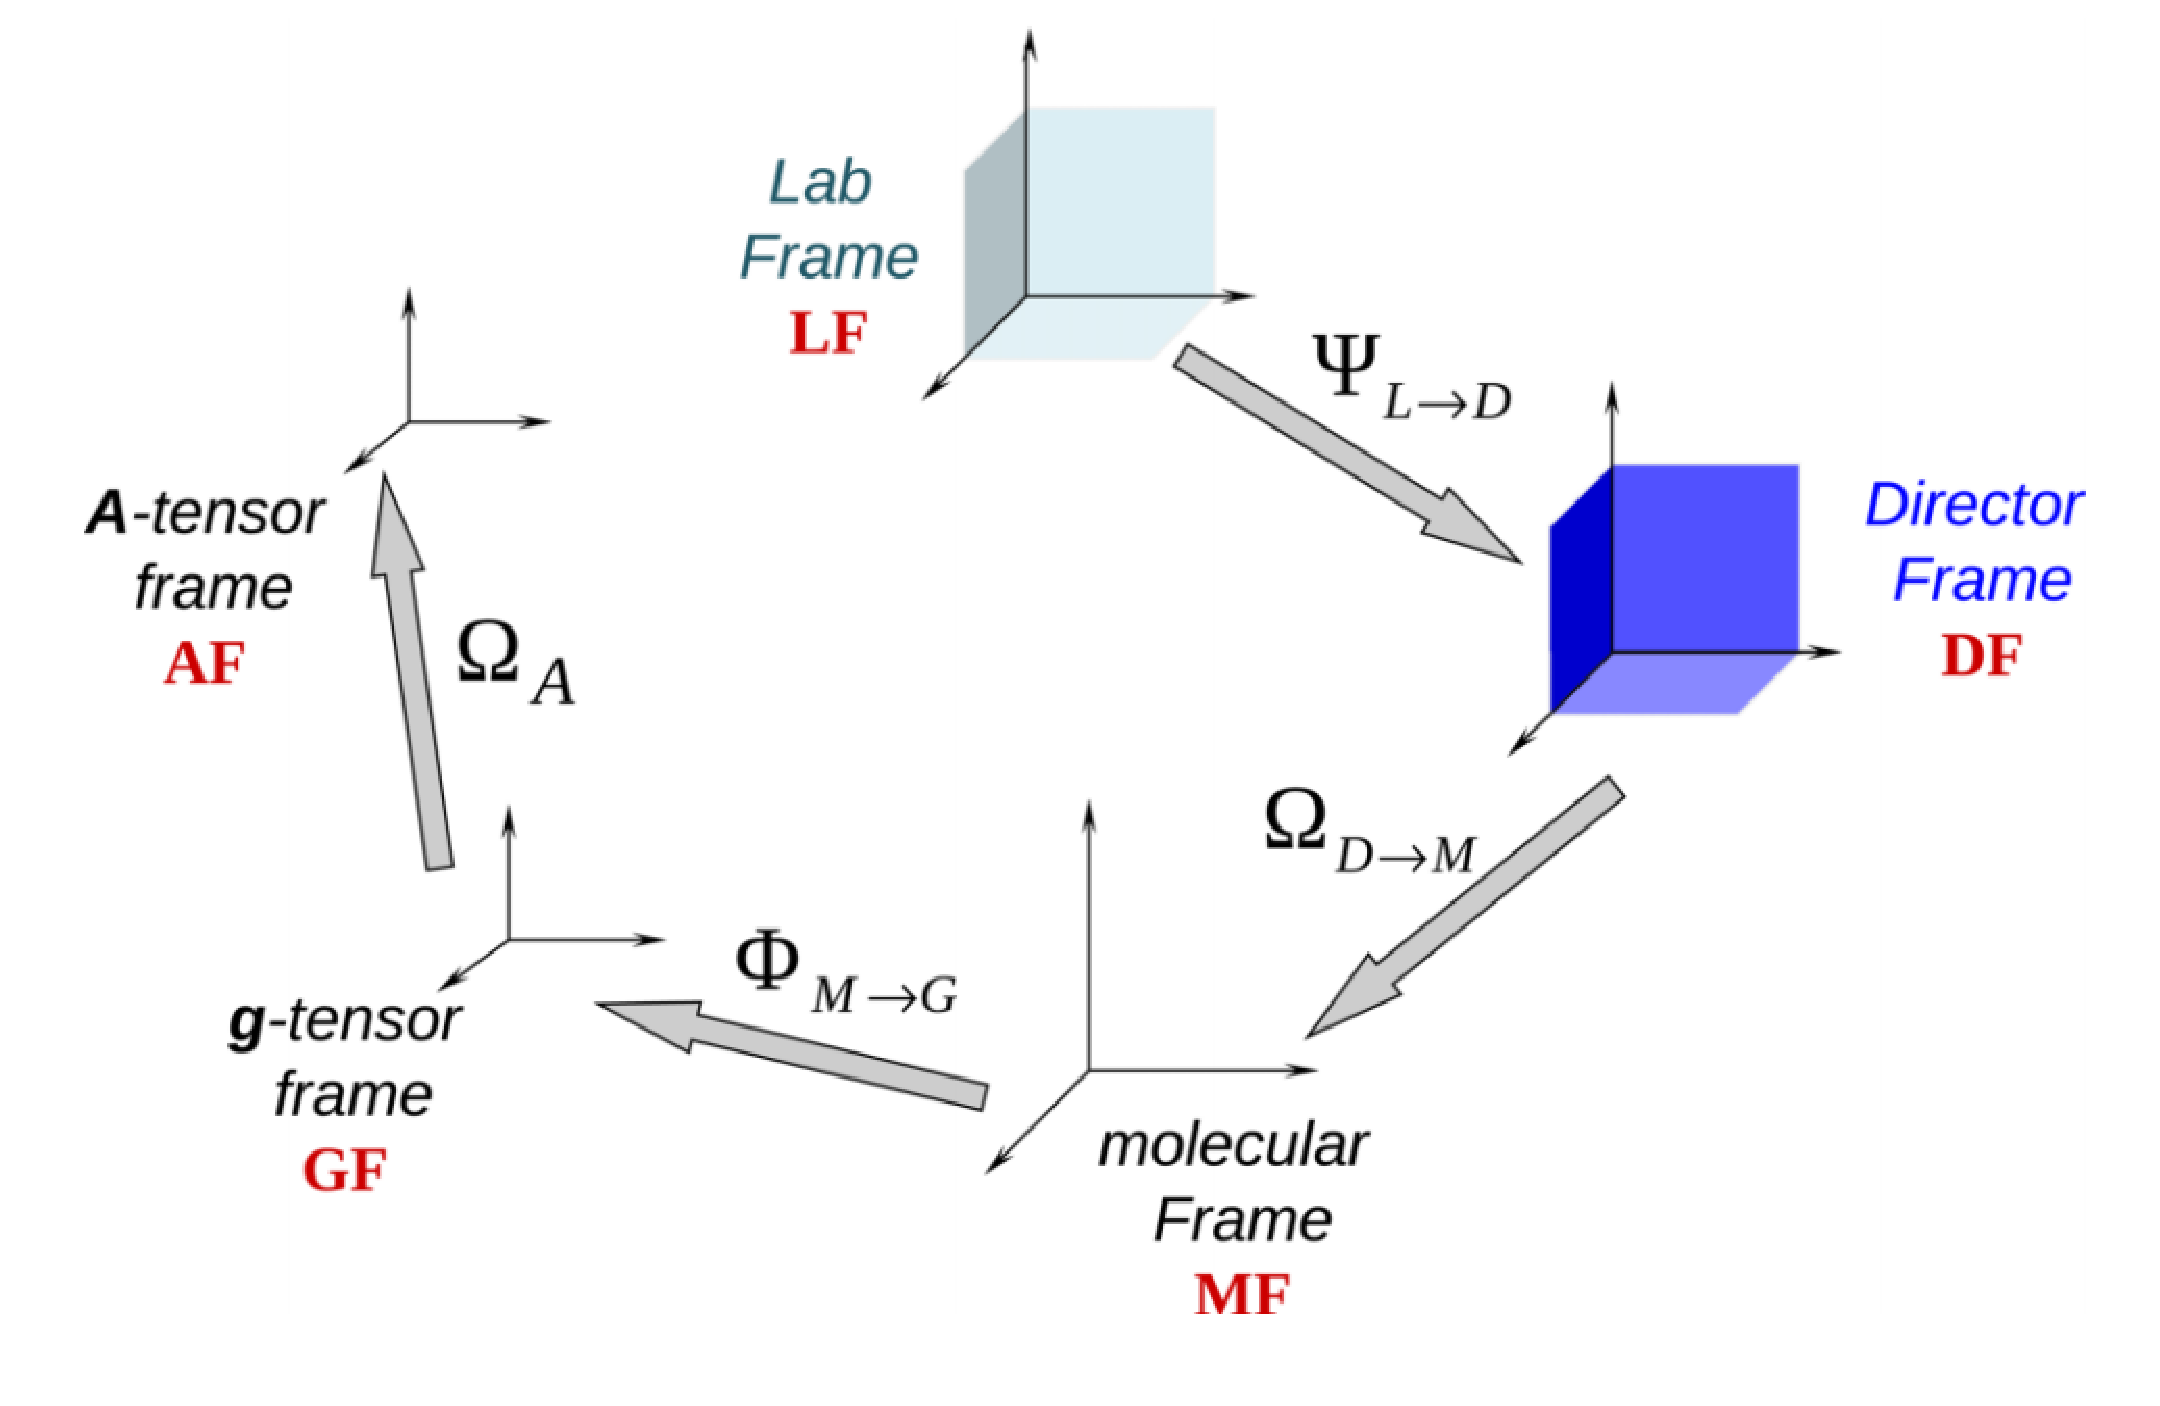
\includegraphics[width=0.7\textwidth]{figures/chap1/frames.eps}
\caption{Example of reference frames that define structural and dynamic properties of the spin-labelled molecules.~\cite{rotat}}
\label{figure:rotat}
\end{figure}
Starting with the detailed construction using Zeeman and Hyperfine interactions it will be shown the powerful use of tensor algebra in magnetic resonance theory:   
\begin{equation}\label{eq:39}
\mathcal{\hat{H}}_{eff}=\hat{S}\cdot g_S\cdot \vec{B}+\hat{S}\cdot A \cdot \hat{I}
\end{equation} 
Space part is represented by $g$ and $A$ tensors that are defined in their own and unique principal axis frames($P$)that are fixed to each other by the molecular frame~\cite{marina}. Magnetic field and spin operators as well as their product are defined in only in a static or laboratory frame. In order to compute EPR spectra or resonance frequencies both tensors have to be defined in the laboratory frame. Rotation of the $g$-tensor to lab frame schematically:  
\begin{equation}\label{eq:40}
 g_{S(P)}\xrightarrow{\textbf{R"}}g_{S(L)}
\end{equation}
Hyperfine tensor $A$ should then rotated into $g$-tensor principal axes and second rotation is done to laboratory frame axes or vice versa. 
\begin{equation}\label{eq:41}
  A_{P}\xrightarrow{\textbf{R'}}A_{g}\xrightarrow{\textbf{R"}}A_{L}
\end{equation}
Here $R', R"$ are rotational matrices that establish mutual orientation between $g$ and $A$ tensors and laboratory frame. There are two ways to treat such rotational transformations between frames. In the first way Cartesian tensors are rotated directly and in second way they are decomposed into irreducible spherical tensor(ISTO) components which are rotating independently and combined back into transformed Cartesian tensor. Spherical tensor operators in three dimensional space have more symmetry features which makes them as more favourable method to use and even more obvious\cite{duer}. The individual spherical tensor components $T_{ml}$ of rank $l$ are given as,     
\begin{equation}\label{eq:42}
  T^{R}_{ml}=\sum_{m'=-l}^lT_{mm'}\mathcal{D}^{(l)}_{mm'}\Omega(\alpha,\beta,\gamma)
\end{equation}
This is analogous to angular momentum basis ket transformation.Rotations in 3-D parametrized by set of Euler equations $\Omega(\alpha,\beta,\gamma)$ transforming stationary $Oxyz$ to a rotational $OXYZ$. Euler angles transformation define orientation of an object in a body-fixed frame to a spaced-fixed of an object. Such transformation is defined by active rotation matrix\cite{bouten}\cite{mul}: 
\begin{figure}[h]
\centering
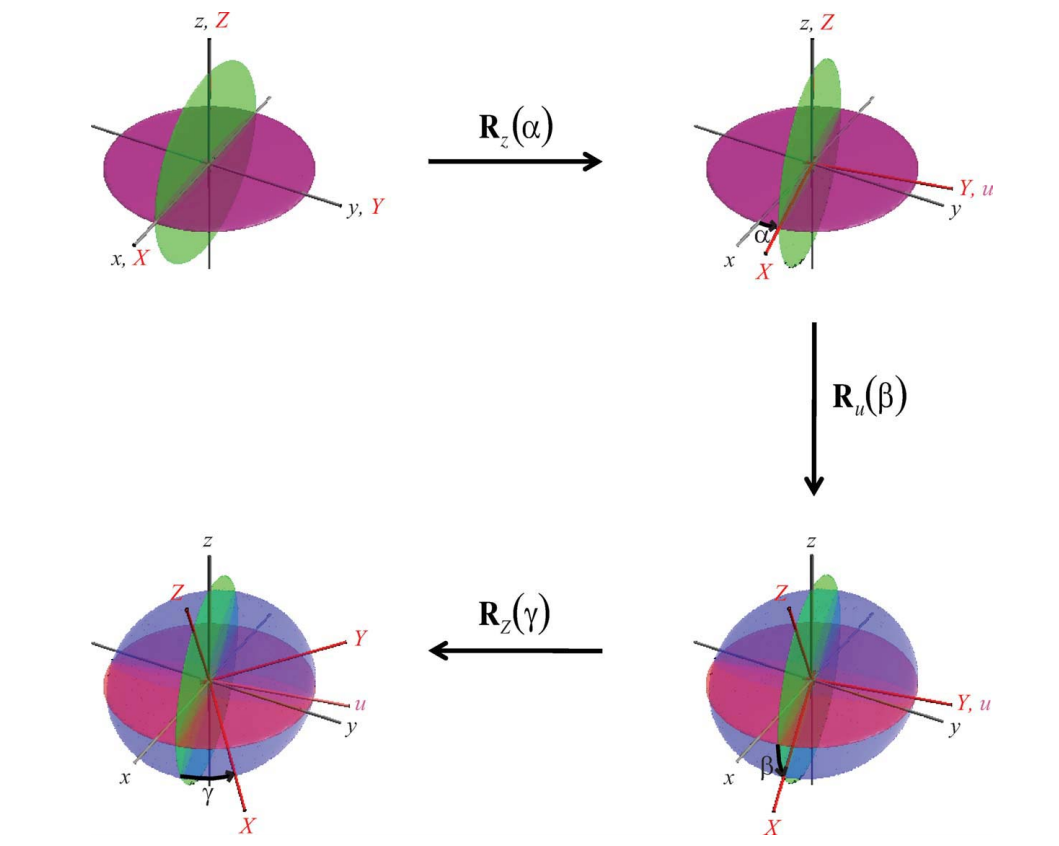
\includegraphics[width=0.7\textwidth]{figures/chap1/rot.png}
\caption{Figure from \cite{mul}}
\end{figure}
\begin{equation}\label{eq:43}
\textbf{R}_A(\alpha,\beta,\gamma) = \begin{bmatrix}
       \cos\alpha \cos\beta \cos\gamma-\sin\alpha \sin\gamma & -\cos\alpha \cos\beta \sin\gamma-\sin\alpha \cos\gamma & \cos\alpha\sin\beta         \\[0.3em]
       \sin\alpha \cos\beta \cos\gamma-\cos\alpha \sin\gamma & -\sin\alpha \cos\beta \sin\gamma-\cos\alpha \cos\gamma & \sin\alpha\sin\beta  \\[0.3em]
       -\sin \beta \cos\gamma & \sin \beta \sin\gamma & \cos \beta
     \end{bmatrix}     
\end{equation}
Transformation back from spaced-fixed frame to body-fixed frame defined by passive rotation transformation matrix $\textbf{R}_P$ and related to active as $\textbf{R}_P(\alpha,\beta,\gamma)=\textbf{R}_A^{-1}(\alpha,\beta,\gamma)$. \\*
Elements $\mathcal{D}_{m,m'}^l$ are known as Wiegner rotation matrix elements and they define expectation values of rotation operator for all magnetic quantum numbers $m$ and $m'$ of the angular momentum $l$ generating rotations~\cite{tomog}: 
\begin{equation}\label{eq:44}
\mathcal{D}_{m,m'}^l=\langle \mathcal{O}(\alpha,\beta,\gamma)\rangle= \langle l,m'|exp(-i\alpha I_x)exp(-i\beta I_y)exp(-i\gamma I_z)|l,m\rangle
\end{equation}
Exponential values with $I_z$ operator can be expanded in Taylor series and evaluated in terms of eigenvalues $m,m'$\cite{brink}. Eq.\ref{eq:44} can be rewritten as:
\begin{equation}\label{eq:45}
\mathcal{D}_{m,m'}^l=exp(-i\alpha I_x)d_{m',m}^{(l)}exp(-i\gamma I_z)
\end{equation}
Where $d_{m',m}^{(l)}$ are reduced Wigner rotation matrix elements. They are real functions and values up to $l=2$ values are given in table \ref{tab:wigner}. Presented table below extremely useful when constructing the full Hamiltonian. 
\begin{table}
\begin{center}
    \begin{tabular}{  l | l }
    \hline
    $d^{l}_{m,m'}$ for $l=1/2,1$ & $d^{l}_{m,m'}$ for $l=2$ \\ \hline
    $d^{1/2}_{1/2,1/2}=d^{1/2}_{-1/2,-1/2}=\cos\frac{\beta}{2}$ & $d^{2}_{2,2}=d^{2}_{-2,-2}=\cos^4\frac{\beta}{2}$ \\
    $d^{1/2}_{-1/2,1/2}=-d^{1/2}_{1/2,-1/2}=\sin\frac{\beta}{2}$ & $\begin{array} {lcl} d^{2}_{2,1} & = & d^{2}_{1,2}=-d^{2}_{1,2} \\ & = & d^{2}_{-1,-2}=-\frac{1}{2}\sin\beta(1+\cos\beta) \end{array}$  \\ 
    $d^{1}_{1,1}=d^{1}_{-1,-1}=\cos^2\frac{\beta}{2}$ & $\begin{array} {lcl} d^{2}_{2,0} & = & d^{2}_{0,2}=-d^{2}_{-2,0} \\ & = & d^{2}_{0,-2}=\sqrt\frac{3}{8}\sin^2\beta \end{array}$ \\ 
    $d^{1}_{1,-1}=d^{1}_{-1,1}=\sin^2\frac{\beta}{2}$ & $\begin{array} {lcl} d^{2}_{2,-1} & = & d^{2}_{1,-2}=-d^{2}_{-2,1} \\ & = & d^{2}_{-1,-2}=\frac{1}{2}\sin\beta(\cos\beta-1) \end{array}$ \\ 
   $\begin{array} {lcl} &d^{1}_{0,1}& =  d^{1}_{-1,0}=-d^{1}_{0,-1}\\ & = & -d^{1}_{1,0}=-\frac{1}{\sqrt{2}}\sin\beta \end{array}$ & $d^{2}_{2,-2}=d^{2}_{-2,2}=\sin^4\frac{\beta}{2}$ \\ 
    $d^{1}_{0,0}=\cos\beta$  & $\begin{array} {lcl} d^{2}_{1,1} & = & d^{2}_{-1,-1} \\ & = & \frac{1}{2}(2\cos\beta-1)(\cos\beta+1) \end{array}$\\ 
     $d^{0}_{0,0}=1$ & $\begin{array} {lcl} d^{2}_{1,-1} & = & d^{2}_{-1,1} \\ & = & \frac{1}{2}(2\cos\beta+1)(1-\cos\beta) \end{array}$ \\ 
      & $\begin{array} {lcl} d^{2}_{1,0} & = & d^{2}_{0,-1}=-d^{2}_{0,1} \\ & = & d^{2}_{-1,0}=-\sqrt\frac{3}{2}\sin\beta\cos\beta \end{array}$ \\ 
      & $d^{2}_{0,0}=\frac{1}{2}(3\cos^2\beta-1)$ \\ \hline
   
    \end{tabular} 
\end{center}
\caption{Algebraic expressions for Wigner rotation matrix elements}
  \label{tab:wigner}
 \end{table}
Hamiltonian is rank zero tensor and thus rotation invariant under coordinate transformation. Using the fact that spherical tensors of the same rank can be contracted the Hamiltonian for the system can be written as~\cite{nordio}:
\begin{equation}\label{eq:46}
  \mathcal{\hat{H}}=\sum_{(int)}\sum_{lm}(-1)^mF_{-m,(int)}^lA_{m,(int)}^l
\end{equation}
where $F_{-m,(int)}$ are components of irreducible spherical tensor describing nature of the interaction and 
$A_{m,(int)}^l$ describe spin operators depending on the type of interaction. $(int)$ decribes the type of interaction(zeeman, hyperfine, dipolar. etc.). 
\begin{equation}\label{eq:47}
  \mathcal{\hat{H}}=\sum_{(int)}\sum_{l,m,m'}(-1)^{m'}F_{-m',(int)}^l\mathcal{D}_{m,m'}(\alpha,\beta,\gamma)A_{m,(int)}^l
\end{equation}
In most general case for the EPR experiments principal axis of $g$ and $A$ tensor even more simplifying  calculations. \\*
It is also useful to use an alternative to Euler angles as under standard parametrization they are non defined at $\beta=0,\pi$. Forgotten pure mathematical technique of quaternions became popular among magnetic resonance community. Geometrically quaternions represent rotation by an angle $\phi$ about an axis determined by the unit vector $\vec{\hat{n}}=\alpha \vec{\hat{i}}+\beta \vec{\hat{j}}+\gamma \vec{\hat{k}}$ and in Euluer-Rodrigues parametrization unit quaternion is give as:
\begin{equation}\label{eq:quat}
\mathcal{A}=\Big[\cos\frac{\phi}{2},\vec{\hat{n}}\sin\frac{\phi}{2}\Big]=[\lambda,\Lambda]
\end{equation}
And terms 
\begin{equation}\label{eq:191}
\lambda=\cos\frac{\phi}{2}
\end{equation}
\begin{equation}\label{eq:191}
\Lambda=\vec{\hat{n}}\sin\frac{\phi}{2}
\end{equation}
Are known as Euler-Rodrigues parameters which give angle-axis parametrization set. To represent stochastic behavour of interaction of spin bath it is also important to map $SU(2)$ to $SO(3)$(hypersphere)~\cite{simon}. This technique is used in order to simulate virtual reality interaction in 3-D~\cite{gorsh}.  

\begin{equation}\label{eq:rquatern}
\textbf{R}(\lambda,\Lambda) = \begin{bmatrix}
       \lambda^2+\Lambda_x^2-\Lambda_y^2-\Lambda_z^2 & 2(\Lambda_x\Lambda_y-\lambda\Lambda_z)  & 2(\Lambda_z\Lambda_x-\lambda\Lambda_y)        \\[0.3em]
       2(\Lambda_x\Lambda_y+\lambda\Lambda_z) & \lambda^2-\Lambda_x^2+\Lambda_y^2-\Lambda_z^2 & 2(\Lambda_y\Lambda_z-\lambda\Lambda_x)  \\[0.3em]
        2(\Lambda_z\Lambda_x-\lambda\Lambda_y)& 2(\Lambda_y\Lambda_z+\lambda\Lambda_x) & \lambda^2-\Lambda_x^2-\Lambda_y^2-\Lambda_z^2
     \end{bmatrix}     
\end{equation}
Where,
\begin{equation}\label{eq:191}
\lambda=\cos\frac{1}{2}\beta\cos\frac{1}{2}(\alpha+\gamma)
\end{equation}
\begin{equation}\label{eq:192}
\Lambda_x=-\sin\frac{1}{2}\beta\sin\frac{1}{2}(\alpha-\gamma)
\end{equation}
\begin{equation}\label{eq:193}
\Lambda_y=\sin\frac{1}{2}\beta\cos\frac{1}{2}(\alpha-\gamma)
\end{equation}
\begin{equation}\label{eq:194}
\Lambda_z=\cos\frac{1}{2}\beta\sin\frac{1}{2}(\alpha+\gamma)
\end{equation}
Wigner matrix elemennts in Euler-Rodrigues parametrization can be written as:
\begin{multline}\label{eq:dlmkeuler}
\mathcal{D}_{m,m'}^l(\lambda,\Lambda)=[(l+m')!(l-m')!(l+m)!(l-m)!]^{1/2}\\ \times \sum_s \frac{(\lambda-i\Lambda_3)^{j+m-s}(-i\Lambda_1-\Lambda_2)^{m'-m+s}(-i\Lambda_1+\Lambda_2)^{s}(\lambda+i\Lambda_3)^{j-m'-s}}{(l+m-s)!(m'-m+s)!s!(j-m'-s)!}
\end{multline}
Eq.\eqref{eq:dlmkeuler} will be used to construct Wigner Matrix and thus gives additional leap on parametrization. 
\clearpage
\subsection{Kubo-Anderson Model of Motional Narrowing}
Spectrum narrowing is known phenomena in magnetic resonance when line shape affected by slow and rapid interaction of the spins with the environment and itself. It takes two forms motional and exchange narrowing. Motional narrowing caused by interactions of atoms in the environment while in motion while exchange interaction affects electronic magnetic moments. Main theoretical work was developed by chemical physicists~\cite{anderson} and ~\cite{kubo} in mid 50's of 20th century. Its relative simplicity and cross-scientific application to different spectroscopic methods ~\cite{inda} attracts more attention and discussion on simulation of complex interacting environment.\\*
First it is important fundamentally define what type of interaction affects the line shape. Non-magnetic interactions have no effect on structural profile as they can not affect relative spins population ratio thus only magnetic like hyperfine, Zeemann or dipolar interaction can have a direct effect. Interestingly that non-magnetic interactions do affect line shape by the localized molecular motions tending to average out and narrow multiplet lines or simply "hide" important structural information on sample like $g$ or $A$ tensors anisotropy. In extreme rapid molecular motion line breadth is defined as~\cite{anderson}: 
\begin{equation}\label{eq:28}
\Delta\omega\simeq \omega_p^2/\tau
\end{equation} 
Where $\omega_p$ frequency of perturbations and $\tau$ is a rate of motion at which narrowing occurs. It is clear from Eq.\ref{eq:28} that adiabatic narrowing can be explained by radiation of electromagnetic wave whose frequency modulated when nuclear or electron spin magnetic begin to precess under environment interaction and frequency changes randomly(stochastically). Originally Kubo~\cite[pp:101-126]{kubo1} attacked the problem of stochastic motion by treating it as $N$ coupled classical oscillators. Frequency of oscillation $\Omega(t)$ of single oscillator at specific coordinate $x(t)$ randomly modulated by the environment and by oscillators themselves. Position of oscillator can be found as: 
\begin{equation}\label{eq:oscill}
x(t)=i\Omega(t)x(t)
\end{equation} 
In stochastic process it is possible to measure amplitude of the modulations $\Delta$ which are defined as:
\begin{equation}\label{eq:harmonoscill}
\Delta=\Big[\int d\Omega p(\Omega)(\Omega)^2\Big]^{1/2}=\langle\Omega^2\rangle^{1/2} 
\end{equation}
Where $p(\Omega)$ is a probability of having a random frequency $\Omega$. The stochastic modulation described as stationary process thus the coherence can be defined as: 
\begin{equation}\label{eq:corellation}
\tau_c=\int_0^{\inf} \frac{\mathrm{d}t\langle\Omega(0)\Omega(t)\rangle}{\Delta^2}
\end{equation}
Integrand in Eq.\ref{eq:corellation} represents correlation function $(G(t)=\langle\Omega(0)\Omega(t)\rangle)$ of the random frequency modulation. Ranges of modulation then are split as: 
\begin{equation}\label{eq:slowmodulation}
\Delta \tau_c \gg 1
\end{equation}
Modulation considered as slow and if: 
\begin{equation}\label{eq:fastmodulation}
\Delta \tau_c \ll 1
\end{equation}
For his work in development of correlation functions R. Kubo received Boltzman Medal~\cite{kubo2} Solution of Eq.\ref{eq:oscill} reduced to finding proper description of the stochastic process. Kubo and Anderson proposed well known approach for describing frequency modulation as Markovian process. In more details Markovian probabilistic process will be discussed later in the chapter. Spectral density or simply line shape for stochastic process is given by: 
\begin{equation}\label{eq:fastmodulation}
I(\omega)=\frac{1}{\pi}\int_0^{\inf}\mathrm{d}t\cos\omega te^{-g(t)}
\end{equation}
Where $g(t)$:
\begin{equation}\label{eq:fastmodulation}
I(\omega)=\int_0^{t}\mathrm{d}t'(t-t')C(t')=\Delta^2\tau t+\Delta\tau^2(e^{-t/\tau}-1)
\end{equation}
For slow modulation regime line shape can be approximated by expanding $g(t)$ in lowest order in $t$ or $g(t)\simeq \Delta^2t^2/2$ which leads to Gaussian line shape: 
\begin{equation}\label{eq:fastmodulation}
I(\omega)=\frac{1}{\sqrt{2\pi\Delta^2}}e^{-\omega^2/2\delta^2}
\end{equation} 
For the fast modulation regime $g(t)\simeq \Delta^2\tau t\equiv t/T_2$ and line shape has a Lorentzian shape: 
\begin{equation}\label{eq:fastmodulationshape}
I(\omega)=\frac{1}{\pi T_2[\omega^2+(1/T_2)^2]}
\end{equation}
So far quantum mechanical aspect of the environment interaction was simplified and classical line shapes narrowing explained only in classical way. From the relaxation spin-lattice relaxation phenomenon it is known that small local oscillating fields create additional transitions between the eigenstates of the system and thus adequate Hamiltonian should be introduced. The model that our group have accepted was developed by Blume ~\cite{blume} and it is known as generalized Kubo-Anderson Model. His approach was essential on development proper time-correlation function to describe phenomenology of both adiabatic and non-adiabatic effects of line shape narrowing. Lets start constructing Hamiltonian for isolated spin nucleus capable of additional transitions and can be presented as: 
\begin{equation}\label{eq:29}
\mathcal{H}(t)=g_N\mu_NB_0I_z+g_N\mu_NhI_zf(t)
\end{equation} 
Where second term that represents fluctuating term due to interaction of the nucleus with the environment. Mathematically problem involves finding solution describe Hamiltonian that randomly changes between finite number of possible states(stochastic) over specified time interval. General form of the Hamiltonian can be represented as: 
\begin{equation}\label{eq:ham}
\mathcal{H}(t)=\sum_jV_jf_j(t)
\end{equation}  
Where terms $V_j$ represent energy information for a physical system and $f_j(t)$ corresponding values of the fluctuation function. Fluctuation function defines "jumps" in time continuous time period. Quantum mechanical treatment can be similar to that of M{\"o}ssbauer spectroscopy to find probability of emission of a photon with a wave vector $\vec{k}$ from transitioning between states $|\lambda\rangle$ and $|\alpha\rangle$ with frequency $\omega$. One can rewrite as:
\begin{equation}\label{eq:30}
P_{\lambda \alpha}(k)=\frac{|\langle \alpha|\mathcal{H}^{(+)}|\lambda\rangle|^2}{(\omega+E_{\alpha}-E_{\lambda})^2+\frac{1}{4}\Gamma^2}
\end{equation} 
Where $\Gamma$ is an inverse of natural lifetime of the excited state. $H^{(+)}$ is describes nucleus interaction with electromagnetic field for emission of a photon. Summarizing over all final states and setting probability of initial event occurring as $p_{\lambda}$ line shape is give in form:
\begin{equation}\label{eq:31}
P(k)=\sum_{\substack{\lambda\alpha}}p_{\lambda}P_{\lambda\alpha}(k)= \left(\frac{2}{\Gamma}\right)Re \int_0^\infty\mathrm{exp(i\omega t-\frac{1}{2}t\Gamma) (\langle \mathcal{H}^{(-)}\mathcal{H}^{(+)}(t) \rangle)_{av} }\,\mathrm{d}t
\end{equation}     
$H^{(-)}=H^{(+)^T}$ are starting vectors and in addition to quantum mechanical average stochastic average denoted as $(...)_{av}$. Time dependence and properties of the system governed by the time evolution operators in quantum mechanical treatment: 
\begin{equation}\label{eq:32}
\mathcal{H}^{(+)}(t)= exp\Bigg[i\int_0^t\mathcal{H}(t')\mathrm{d}t'\Bigg]\mathcal{H}^{(+)}exp\Bigg[i\int_0^t\mathcal{H}(t')\mathrm{d}t'\Bigg]
\end{equation}  
Stochastic states defined by the Markovian process and treatment is similar to Kubo~\cite{kubo1}. Fundamental result for our group can be described by the final result of Blume theoretical calculations. Line shape defined as: 
\begin{multline}\label{eq:33}
P(\omega)=
\frac{2}{\Gamma(2I_0+1)}\sum_{\substack{m_1m_0,m_{1'}m_{0'}}}\langle I_1m_1|\mathcal{H}^{(-)}|I_0m_0\rangle\\\sum_{\substack{ab}}p_a\langle I_0m_0I_1m_1a|\mathcal{L}^{-1}|I_0m_0'I_1m_1'b\rangle \langle I_0m_0'|\mathcal{H}^{(+)}|I_1m_1'\rangle
\end{multline}
In this expression $I_0$ is a nuclear spin of ground state and $I_1$ spin of excited state,$a$ and $b$ represents stochastic states defined by function $f(t)$ and $p_a$ is an a priory probability of stochastic transition occurrence between states. $\mathcal{L}$ is a Liouville super matrix that was described before. Terms 
$\langle I_1m_1|\mathcal{H}^{(-)}|I_0m_0\rangle $ and $\langle I_1m_1|\mathcal{H}^{(-)}|I_0m_0\rangle $ can be found in terms of Glebsh-Gordan coefficients. Given form of the line shape calculation represents the case of NMR but changing nuclear operators to electron spin operators or quantum states will represent the case of isolated free electron spin resonance or EPR. In case of coupled interaction of spin to nucleus Eq.\ref{eq:33} can be easily extended with little algebra work. Construction of Liouville superoperator $\mathcal{L}$ is simmilar to previous subsection but with minor updates: 
\begin{equation}\label{eq:34}
\mathcal{L}=p(\omega)\hat1 - W-i\sum_jV_j^{\times} F_j
\end{equation}
Problem of using Eq.\ref{eq:33} is to take assign and take matrix inverse of the Liouville array$(\mathcal{L}_{a,m_0,m_1,b,m_0',m_1'})$ that is also defined by superoperator acting on nuclear or/and electron spin quantum states: 
\begin{equation}\label{eq:35}
\mathcal{L}_{a,m_0,m_1,b,m_0',m_1'}=\Big[\langle I_0m_0I_1m_1a|p(\omega)\hat1 - W-i\sum_jV_j^{\times} F_j|I_0m_0'I_1m_1'b\rangle\Big]^{-1}  
\end{equation}
The size of Liouville matrix defined as $(2I_0+1)(2I_1+1)n$ for isolated nuclear spin or in case of both NMR and EPR treatment size is specified as $(2I_0+1)(2I_1+1)(2S_0+1)(2S_1+1)n$
and $n$ is a number of stochastic states. For example if considering only nuclear spin-1/2 and  assuming that $I_0=I_1$, n=2 we get matrix of a size $8\times 8$ and if electron spin-1/2 interaction is considered along with nuclear the size becomes $32\times 32$. $W$ matrix is known as transition rate matrix and its elements are defining rates of transition between stochastic states. More details on assignment $W$ matrix will be provided later and it plays important role in describing motional adiabatic effects. The first term is a frequency $p(\omega)=i(\omega+0.5i)$ where $0.5i$ is added for line shapes not to collapse on delta peaks. $V^{\times}_j$ is a Liouville super-operator defined similarly as in Eq.\ref{eq:ham} : 
\begin{multline}\label{eq:36}
\langle I_0m_0I_1m_1a|V^{\times}_j|I_0m_0'I_1m_1'b\rangle= \\
\delta_{ab}[\langle I_0m_0|V_j|I_0m_0'\rangle \delta_{m_0m_ 0'}-\langle I_1m_1|V_j|I_1m_1'\rangle \delta_{m_1m_1'}]
\end{multline}
In order to simplify Eq.\ref{eq:33} for readable computational description  in terms of delta Kronecker it can be rewritten as: 
\begin{multline}\label{eq:37}
P(\omega)=
\frac{2}{\Gamma(2I_0+1)}\mathcal{H}^{(-)}\delta_{m_1m_0}\mathcal{H}^{(+)}\delta_{m_0'm_1'} \ [s\delta_{ab}\delta_{m_1m_1'}\delta_{m_0m_0'} \\-(a|W|b)\delta_{m_0m_0'}\delta_{m_1m_1'} \\ -i(a|F|a)\delta_{ab}[\langle I_0m_0|V_j|I_0m_0'\rangle \delta_{m_0m_ 0'}-\langle I_1m_1|V_j|I_1m_1'\rangle \delta_{m_1m_1'}]^{-1}
\end{multline}   
Computationally Problem reduces to finding algorithm of populating multidimensional arrays in Liouville vector space and physically is to define proper energy representation of the system and add all interaction terms to final Hamiltonian.     
\clearpage 
\chapter{Model Development and Results}
\section{Results Magnetic Resonance}
We will discuss algorithmic approach on developing the generalized Kubo-Anderson model. We will describe general computational pitfalls that was faced during the software development and proposed solutions and tools to simulate stochastic behavior of the interacting systems in applied magnetic field. The introduction to Masters equation and transition rate matrix construction will be covered as well. At the end of the chapter we will cover Hamiltonian construction and difference between various models in low and high field approximations.
\subsection{Algorithm to find inverse of Liouville Matrix}\label{algorithmsection}
In order to obtain lineshape from stochastic approach on relaxation effects of spin dynamics it is important to asset proper inversion algorithm of Liouville matrix from Eq\.Ref{eq:35}. Liouville matrix can be represented as two dimensional array where each index of the dimension has and additional three sub-indexes specified by stochastic and electron or/and nuclus spin states. In other words: 
\begin{equation}\label{eq:53}
\mathcal{L}_{i,j}=\mathcal{L}_{a,m_0,m_1;b,m_0',m_1'}  
\end{equation}  
Where $i\rightarrow a,m_0,m_1$ and $j\rightarrow b,m_0',m_1'$. Computationally there are two distinctive approaches on populating and inverting the matrix. In the first approach Liouville matrix kept two dimensional and general rule on encoding each index into three sub-indexes should be elaborated. This task is ambiguous and probability of undiscovered omission while perfect compilation is high. From the second approach Liouville two dimensional matrix can be deployed into higher dimensions where each dimension is specified according to quantum and stochastic states:  
\begin{equation}\label{eq:54}
\mathcal{L}_{i,j}=\mathcal{L}_{a,m_0,m_1;b,m_0',m_1'}\rightarrow \mathcal{L}_{a,m_0,m_1,b,m_0',m_1'}
\end{equation}
The need of such transformation is to simplify assignment of Liouville matrix according to the action of spin operators on quantum states and tracking of stochastic states. Also it will simplify summation that have to be performed in order to compute line shape from Eq. 33. Access of matrix elements of dimensions higher than 2 can be illustrated through concept of the "page" representation on fig. 4. 
\begin{figure}[h!]
\centering
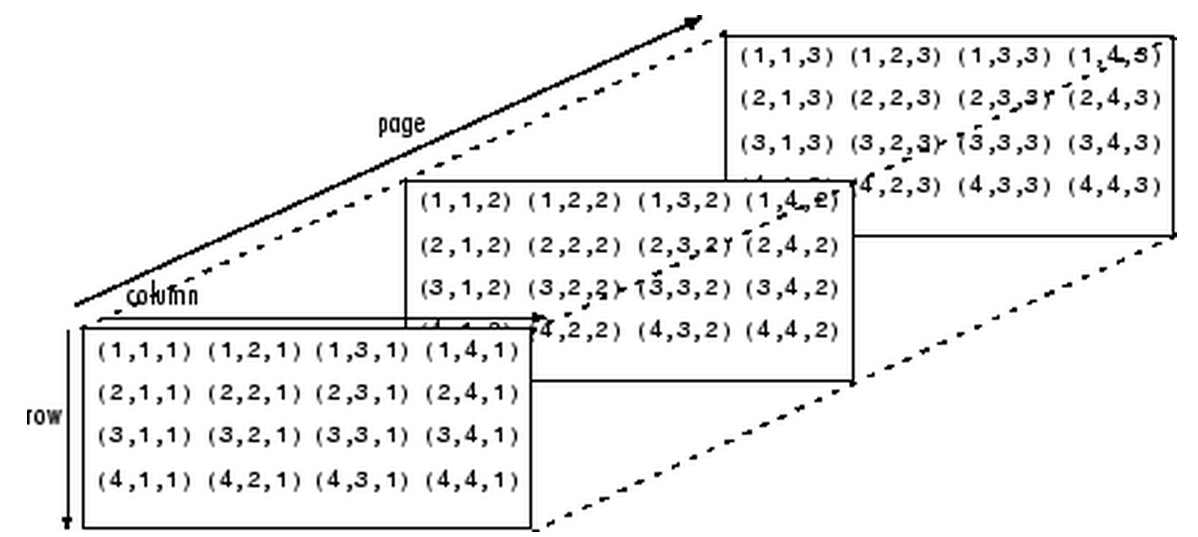
\includegraphics[width=0.7\textwidth]{figures/chap1/mat.png}
\caption{Illustration of "page" concept of storing and accessing elements of 3-dimensional array $A_{4,4,4}$ or $A[4,4,4]$ with four elements in each dimension.~\cite{Matlab}}
\end{figure}
\\
For example Liouville matrix for isolated nuclear spin has six dimensions $\Big(\mathcal{L}[a,m_0,m_1,b,m_0',m_1']\Big)$ and if electron spin interaction is added it expands to overall ten dimensions specified by four additional sub-indexes $m_{0S},m_{1S},m_{0S}',m_{1S}'$ or $\Big(\mathcal{L}[a,m_{0S},m_{1S},m_0,m_1,b,m_{0S}',m_{1S}',m_0',m_1']\Big)$. \\
Issue arises from the fact that matrix inversion of the multidimensional array is limited to finding inverse of every specified "page" rather then whole array structure. Transition from higher dimensions to dimension where it is possible to perform matrix inversion is important step in computational algorithm. While transforming from N-dimensions to two dimensions where matrix inverse can be found it is important to track the indexes transformation. In order to achieve proper index transformation a hash table should be created. \\*
 Example of hash table for the case where $a=b=4$, $m_0=m_0'\pm1/2$ and $m_1=m_1'\pm1/2$ implemented in Java is given at table \ref{table:kysymys}. 

\begin{table}[h!]
\begin{center}
    \begin{tabular}{  l  l  l  l l }
    \hline
    $a,m_0,m_1$ &  & Output & Key\\ \hline
    $1,1/2,1/2$ & $\rightarrow$ & 000 & 1 \\ \hline
    $1,-1/2,1/2$ & $\rightarrow$ & 010 & 2  \\ \hline
    $1,1/2,-1/2$ & $\rightarrow$ & 001 & 3 \\ \hline
    $1,-1/2,-1/2$ & $\rightarrow$ & 011  & 4\\ \hline
    $2,1/2,1/2$ & $\rightarrow$ & 100 & 5 \\ \hline
    $2,-1/2,1/2$ & $\rightarrow$ & 110 & 6  \\ \hline
    $2,1/2,-1/2$ & $\rightarrow$ & 101 & 7 \\ \hline
    $2,-1/2,-1/2$ & $\rightarrow$ & 111  & 8\\ \hline
    $3,1/2,1/2$ & $\rightarrow$ & 200 & 9 \\ \hline
    $3,-1/2,1/2$ & $\rightarrow$ & 210 & 10  \\ \hline
    $3,1/2,-1/2$ & $\rightarrow$ & 201 & 11 \\ \hline
    $3,-1/2,-1/2$ & $\rightarrow$ & 211  & 12\\ \hline
    $4,1/2,1/2$ & $\rightarrow$ & 300 & 13 \\ \hline
    $4,-1/2,1/2$ & $\rightarrow$ & 310 & 14  \\ \hline
    $4,1/2,-1/2$ & $\rightarrow$ & 301 & 15 \\ \hline
    $4,-1/2,-1/2$ & $\rightarrow$ & 311  & 16\\ \hline

    \end{tabular}
\end{center}
\caption{Hash table of Liouville matrix $i$-th index for Java and Python}
\label{table:kysymys}
\end{table}

In general the same pattern of encoding is valid for $j$-th index that consists of $b,m_0'$ and $m_1'$ if $I_0=I_1$ or $S_0=S_1$ but not necessary $S_0=I_0$ or $S_1=I_1$. Main requirement that transformed two dimensional matrix should be square and number of elements should be the same as of multidimensional. Transformation from N-dimensional to 2-dimensional is possible through for-loops control statements. Encoded index stored as double rather then string which ads up complexity on extracting the index when needed but performance wise is better. Each indexes specified by stochastic and quantum states are saved as their total combination in hash table as a string and unique key is being assigned. By the unique key assigned to each element of 2-dimensional array each of the corresponding indexes of multidimensional array can be restored after conversion. Core concepts of the inversion algorithm are possible to divide into 4 important stages:  

\begin{center}
\begin{enumerate}
\item Assign Liouville multidimensional matrix: $\mathcal{L}[a,m_0,m_1,b,m_0',m_1']$
\item Transform multidimensional matrix into 2-dimensional: $\mathcal{L}[a,m_0,m_1,b,m_0',m_1'] \rightarrow \mathcal{L}'[i,j]$ 
\item Transformed matrix inversion: $\mathcal{L}'[i,j]=\mathcal{L}'[i,j]^{-1}$
\item Transformation 2-dimensional matrix back to multidimensional: \\ $\mathcal{L}'[i][j]\rightarrow \mathcal{L}[a,m_0,m_1,b,m_0',m_1']$ 
\end{enumerate}   
\end{center}    
Stage 4 is important as it simplifies summation defined by Eq. 36. \\*
In order to establish algorithm implementation as well as proceeding software developing Java, Matlab and Python have been tested on computational efficiency. \\*
Java is  a programming language released by Sun Microsystems in 1995. It is a object-oriented programming language and distributed freely and portable on most modern operating systems platforms. Classes define objects constructors and represent interfaces in a Java application. Just In Time compiler(JIT) bring a boost to queries and computational efficiency allowing to track productivity of each separate part of code~\cite{hortell} and in Java 8 parallel execution of classes have been added~\cite{javapal}. In Java multidimensional arrays represented as an N-dimensional Object superclass and part of java.util.Arrays package. Any interaction between Objects in Java is valid if they are define through the methods that are specified for both objects. For complex numbers operations Thomas Flanagan~\cite{flanagan} Scientific Library was used. Author of this dissertation finds counterproductive rewriting basic available as open source linear algebra packages and relies on 3-d party developers as true example fo scientific collaboration. For the visualization properties for 2-D chats JFreeChart based on native Java Foundation Classes(JFC). For 3-D visualisation Jzy3d open source library was used that requires Open Graphics Library(OpenGL)  multi-platform application programming interface for rendering vector graphics.\\*
As a result we have written SpinAl software based on the described algorithm. It has natively simple interface and comes as SpinAl.jar file. It can be launched on any machine with the Java 7+ environment installed. On MacOS and Linux you can either double tap on the jar-file or to use terminal to launch it:
\begin{lstlisting}
$ java -jar SpinAl.jar
\end{lstlisting}
The main menu on Fig.\ref{figure:SpinAl1} will pop up asking to specify the stochastic values $a$ and $b$ as well as frequency range. Proceeding menu on Fig.\ref{figure:SpinAl2} will require to enter precise details on the values of fixed and fluctuating magnetic fields based on Hamiltonian described by Eq.\eqref{eq:blumeham}. Also transition rate have to be specified. We expect stochastic numbers are symmetric thus exception will be thrown if $a\neq b$. 
\begin{figure}[h!]
\centering
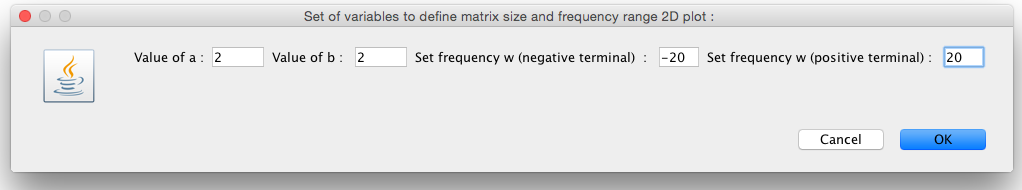
\includegraphics[width=0.8\textwidth]{figures/chap2/spinal1.png}
\caption{Main menu of the SpinAl software with parameters selection for stochastic indexes and frequency range.}
\label{figure:SpinAl1}
\end{figure}
For this specific example we set $a$ and $b$ as 2. Frequency range as $-20\leq\omega\leq 20$. Fixed magnetic field as 4 and fluctuating magnetic field along z-axis with a value of 3. transition rate value was randomly chosen as 0.01. We will describe in more details why this parameters were used and more details on the Hamiltonian derivation and Lioville matrix population at section\ref{blumeinitialmodel} 
\begin{figure}[h!]
\centering
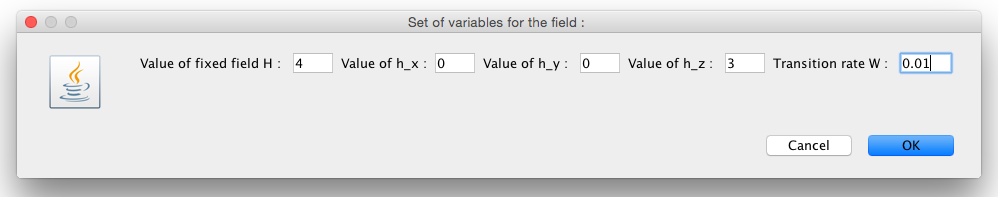
\includegraphics[width=0.8\textwidth]{figures/chap2/spinal2.png}
\caption{Proceeding menu of the SpinAl software with parameters selection for applied and fluctuating magnetic field as well as transition rate $W$.}
\label{figure:SpinAl2}
\end{figure}
\begin{figure}[h!]
\centering
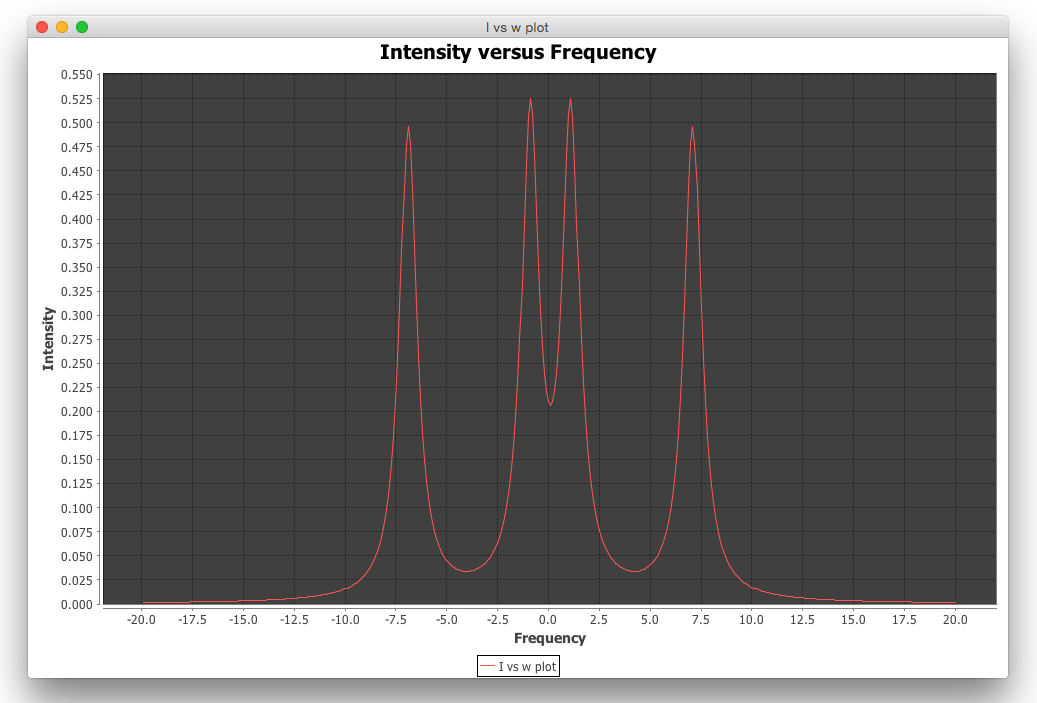
\includegraphics[width=0.8\textwidth]{figures/chap2/spinal3.png}
\caption{Produced graph of the Intensity versus Frequency after all model parameters have been entered.}
\label{figure:SpinAl3}
\end{figure}
Output of the computation will be Intensity versus frequency graph as on Fig.\ref{figure:SpinAl3}. \\
Currently SpinAl limited 2, 6 and 48 stochastic indexes as transition rate matrix under rotations is developed for this specific cases. We plan to generalize the software in future releases by adding possibility of creating custom $W$-matrix as well as rotation angles that could be uploaded as text files and parsed by SpinAl. Source code is available at authors public GitHub repository under open license\cite{nmrgit}.\\
The core algorithm of SpinAl to invert N-d arrays has been separated into framework available on separate GitHub repository\cite{ndgit}. It supports up to 10-D complex arrays inversion. Maximum size supported arrays size is limited precisely as: \ Array[100][100][10][10][10][10][10][10][10][10].\\
While working on SpinAl during mine PhD career our group was also exploring another possibilities to make computations cost-efficient. Thus we have successfully ported SpinAl to Python programming language where N-d array inversion was overcome by using native methods from scientific libraries. Python is a multi-paradigm high level cross-platform programming language that is well known for its relative simplicity of the syntax and fast expanding open source committing community. It is slower then Java~\cite{slower}. Core libraries like NumPy and SciPy \cite{scipy} for linear algebra make it relatively fast to perform system prototyping~\cite{SciPy1}~\cite{SciPy2}. Algebraic manipulations on N-Dimensional arrays are available in NumPy \cite{numpy} and two different algorithms on reshaping arrays in Fortran-like and C-like are available. Most of the well used libraries written for purpose of Magnetic Resonance computer simulations are given in Fortran code and using Python code wrapper it is possible to efficiently use the out of the box. We have also explored possibility of GPU~\cite{gpu} as well. The key results of this work will be mostly done in Python.\\*
We have also developed numerous useful tolls for proof-of-concept as well as transition rate matrix population in Matlab which are available upon request from Professor Keith Earle Lab. Matlab is a widely know in computational community multi-paradigm proprietary language developed by MathWorks and requires licence to use it. Matlab 8.2 R2013B was used to for the SpinAl algorithm implementation as well but had a lower performance to the equivalent in written Java. Using C-like N-dimensional array inversion available in latest releases I was not able to reproduce generalized results as in Java and Python in high magnetic field and lower transition rates regimes. Thus majority of the discussed results were obtained in Java and mostly in Python. Python source code is available at GitHub repository as well~\cite{eprgit}\\*
For computation purposes Asus ROG G75VX laptop was used with Intel 3rd generation Core i7 3630QM  processor, 16 GB DDR3 1600GHz memory and equipped with NVIDIA GTX 670 MX graphic processing unit(960 cores).\\* 
\subsection{Transition Rate Matrix}\label{trmsection}
In order to advance in description of the interacting environment well discussed in section \ref{kuboandersonsection} we need to determine suitable number of stochastic states $a$ and $b$ that form a two dimensional matrix $W$ known as transition rate matrix. We will start introduction from pure probabilistic approach with correlation to spin dynamics. We were discussing computational algorithm performance in a previous section but have not yet established the relation between 2,6 and 48 sotchastic indexes and their significance. Our goal in this research work was to determine lower bound of discrete states that are necessary to faithfully reproduce an ESR lineshape using concepts derived from information geometry\cite{Earle2009}.\\*
We start by exploring any physical system with two states as an example electron or nucleus spin-1/2 systems with possible spin up or down orientations.   
\begin{equation}\label{eq:master}
\frac{dp_{i}}{dt}=-\sum_{j\neq i}w_{i\rightarrow j}p_{i}+\sum_{j\neq i}w_{j\rightarrow i}p_{j}
\end{equation}   
\begin{equation}\label{eq:masterbal}
w_{i\rightarrow j}p_{i}=w_{j\rightarrow i}p_{j}
\end{equation} 
\begin{equation}\label{eq:matrix}
\frac{d\vec{p}}{dt}=-\vec{W}\vec{p}
\end{equation} 
Where $\vec{p}$ is a column vector with probabilities $p_i$ and $\vec{W}$ is a square transition rate matrix.

Just as with discrete time, a continuous-time stochastic process is a Markov process if the conditional probability of a future event given the present state and additional information about past states depends only on the present state. A CTMC is a continuous-time Markov process with a discrete state space, which can be taken to be a subset of the nonnegative integers.\\*
\begin{equation}\label{eq:markov}
P(X(s+t)=a|X(s)=b,X(r)=a_r,r\in A_s\subset[0,s))=P(X(s+t)=b|X(s)=a)
\end{equation}   
for all states $i$ and $j$ and for all times $s > 0$ and $t > 0$. On the left in \ref{eq:markov}, we are conditioning on the values of $X(r)$ for all times $r$ in a subset of “past” times $A_s$ in addition to the value at the “present” time $s$. In general, $A_s$ could be an arbitrary subset of $[0, s) \equiv (r:0\leq r<s)$,but to have the conditional probability in \ref{eq:markov} well defined by elementary methods, we assume that $A_s$ is a finite subset. \\*
The conditional probabilities $P(X(s+t) = j|X(s) = i)$ are called the transition probabilities. We will consider the special case of stationary transition probabilities (sometimes referred to as homogeneous transition probabilities), occurring when
\begin{equation}\label{eq:markov}
P(X(s+t)=a|X(s)=b)=P(X(t)=b|X(0)=a) \equiv P_{i,j}(t)
\end{equation} 
Just as in discrete time, the evolution of the transition probabilities over time is described by the Chapman-Kolmogorov equations, but they take a different form in continuous time. In
formula (2.4) below, we consider a sum over all possible states at some intermediate time. In doing so, we simply write a sum over integers. When we do that, we understand the sum to be over all possible states.
\begin{equation}\label{eq:markov}
P_{i,j}(s+t)= \sum_k P_{i,k}(s)P_{k,j}(t)
\end{equation} 
A second modelling approach is based on representing the transition probabilities as the solution of a system of ordinary differential equations, which allows us to apply well-established modelling techniques from the theory of differential equations in a deterministic setting; e.g.,see Simmons (1991).But first we must define zero-time transition probabilities, which we do in the obvious way: We let $P(0) = I$, where $I$ is the identity matrix; i.e., we set $P_{i,i}(0) = 1$ for all $i$ and we set $P_{i,j} (0) = 0$ whenever $i \neq j$. We are just assuming that you cannot go anywhere in zero
time. We then let the transition rate from state $i$ to state $j$ be defined in terms of the derivatives:
\begin{equation}\label{eq:markov3}
W_{i,j}\equiv P_{i,j}'(0)\equiv \frac{dP_{i,j}}{dt}
\end{equation} 
For a finite state space, which we have assumed, and for infinite state spaces under extra regularity conditions, we will have
\begin{equation}\label{eq:markov3}
-W_{i,i}\equiv\sum_{j,j\neq i}W_{i,j}
\end{equation} 
As an example of transition rate matrix construction one can assume two possible random events occurrence. In terms of magnetic resonance this situation is close to chemical shifts and will be discussed in a bit more details later.  
\begin{equation}\label{eq:55}
W = \begin{bmatrix}
       -w_{11} & w_{12}  \\[0.3em]
        w_{21} & -w_{22}  
     \end{bmatrix}
\end{equation}
Diagonal elements are defined via Eq.\ref{eq:markov3} and it means that probability leaving the state is equal to the probability of reaching it. In more complicated example whn relaxation processes couples more states due to the complicated spin motion pattern consider 6 possible states(events). Graph of allowed transitions is given on Fig.\ref{figure:wdiagramm}. One can imagine an octahedron in three dimensional representation labelling edges with indexes from 1 to 6 and defining adjacency matrix of relative coupling,    
\begin{figure}[h!]
\begin{center}
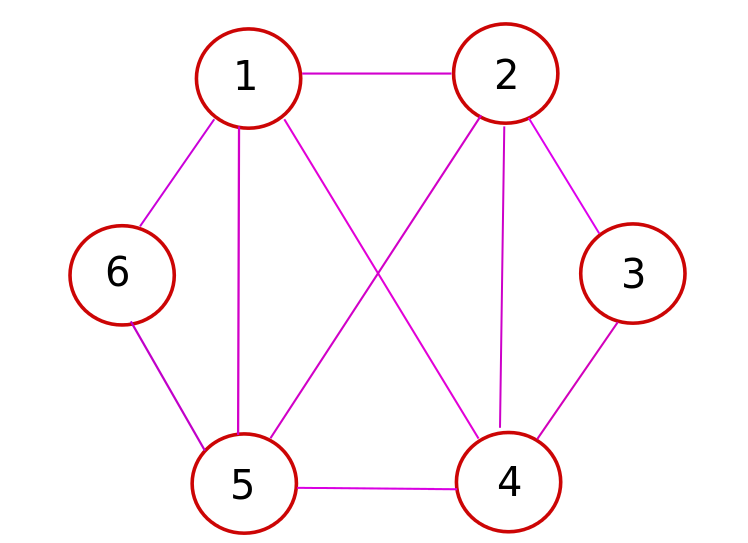
\includegraphics[width=0.7\textwidth]{figures/chap2/wdiagramm.png}
\caption{transition probabilities graph between 6 possible events}
\label{figure:wdiagramm}
\end{center}
\end{figure}
\begin{equation}\label{eq:Wmat1}
W = \begin{bmatrix}
       w_{11} & w_{12} & 0 & w_{14} & 0 & w_{16}  \\[0.3em]
       w_{21} & w_{22} & w_{23} & 0 & w_{25} & 0  \\[0.3em]
       0 & w_{32} & w_{33} & w_{34} & w_{35} & 0  \\[0.3em]
       w_{41} & 0 & w_{43} & w_{44} & w_{45} & 0 \\[0.3em]
       0 & w_{52} & 0 & w_{54} & w_{55} & w_{56} \\[0.3em]
       w_{61} & 0 & w_{63} & 0 & w_{65} & w_{66} 
     \end{bmatrix}
\end{equation}
Diagonal elements are defined as well as for 2 events case by Eq.\ref{eq:markov3}. Another interest is to define rate of tumbling between probability of transitions and assume that an a priori probability between different states transitions might not equal to each other. More evidentially assume transformation of principal axis frame of $g$ or $A$ tensors that are parametrized by euler angles and define  fast transition as $\vec{R}(0,0,0)\xrightarrow {1\rightarrow 6}\vec{R}(0,0,\pi/2)$. Similarly moderate $\vec{R}(0,0,0)\xrightarrow {1\rightarrow 2}\vec{R}(0,\pi/2,0)$  and slow $\vec{R}(0,0,0)\xrightarrow {1\rightarrow 4}\vec{R}(0,0,\pi/2)$. The results for the constructed matrix is given below,   
\begin{equation}\label{eq:Wmat2}
W = \begin{bmatrix}
       0 & m & 0 & s & 0 & f  \\[0.3em]
       m & 0 & s & 0 & f & 0  \\[0.3em]
       0 & s & 0 & f & m & 0  \\[0.3em]
       s & 0 & f & 0 & m & 0 \\[0.3em]
       0 & f & 0 & m & 0 & s \\[0.3em]
       f & 0 & m & 0 & s & 0 
     \end{bmatrix}
\end{equation}
Where $s,m$ and $f$ define three probability transition rates: slow, moderate and fast respectively. It appears that for special cases it might slightly modify the line shape. Yet another even more complicated case is given as 48 total stochastic states defined by quaternion representation by rotation by $\pi/2$ on $S(3)$ assuming nearest neighbours distance as $pi/4$ and Euler angles have been reconstructed. The output of the adjacent matrix is appeared to be sparse
\begin{figure}[h!]
\begin{center}
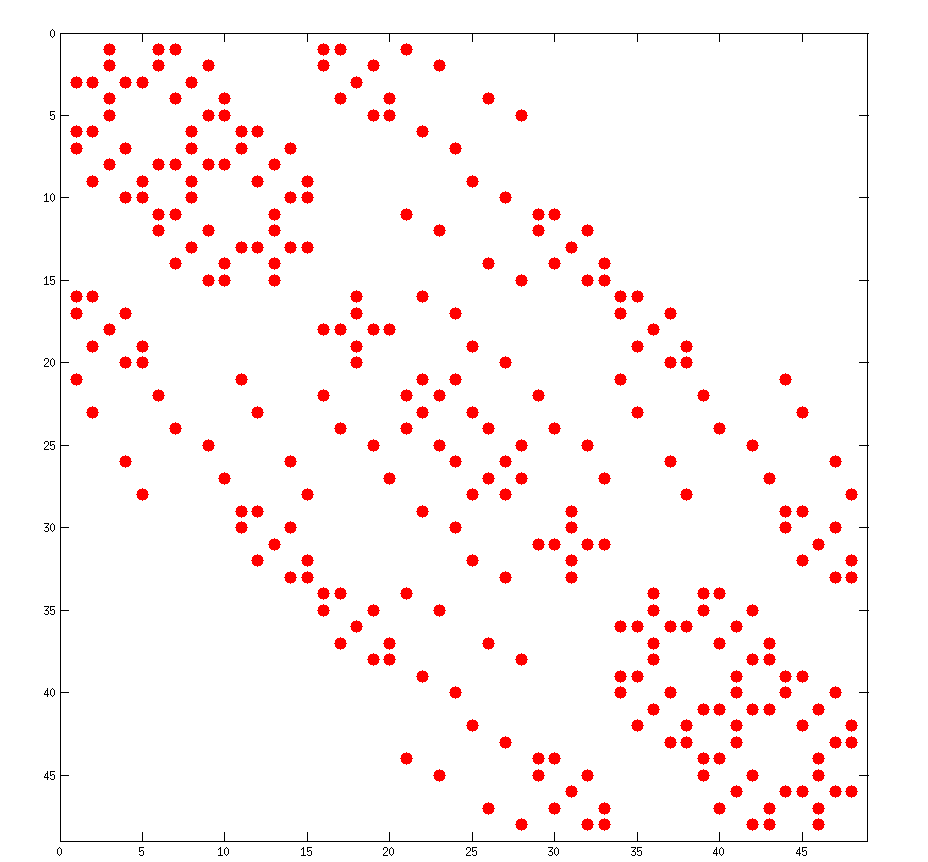
\includegraphics[scale=0.5]{figures/chap2/sparce.png}
\caption{Illustration of allowed transitions between 48 states defined by quaternion representation of  rotation os $S(3)$. Allowed transitions are in red. }
\label{figure:blumediag}
\end{center}
\end{figure}  
\clearpage
\subsection{Chemical Shift}\label{blumeinitialmodel}
Validation step for validation AI algorithm is to reproduce original absorption spectra of NMR linehshape for isolated spin-1/2 nucleus in a fixed magnetic field and fluctuating fields along $x,y$ and $z$ orientations. For specific model $I_0=I_1=1/2$. Number of stochastic states corresponds to two and can be described as chemical exchange process. As simple example of chemical exchange consider two $N$-methyl groups in $N,N'$ - dimethylformamide can exchange their relative bond and reactant chemically and physically remains indistinguishable from the product. Methyl groups are coloured in red and black to make process visible.       
\begin{figure}[h!]
\centering
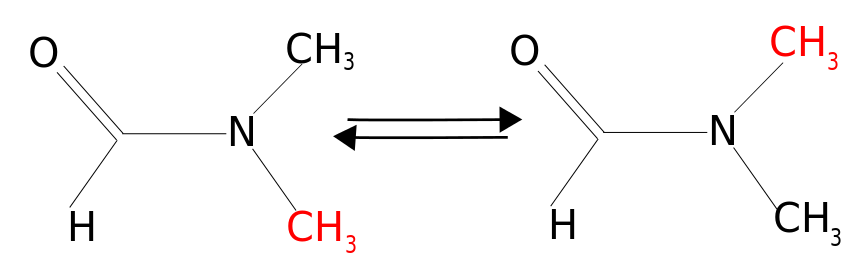
\includegraphics[width=0.7\textwidth]{figures/chap2/methil.png}
\caption{$N,N'$ -
dimethylformamide chemical exchange of methyl groups in active moiety.}
\label{figure:methyl}
\end{figure}
Magnetic environment of $N$-methyl groups will be different after the chemical exchange which leads to the fact that they will have different resonance frequencies before and after the reaction and molecular motion can be treated by Blume stochastic model. Example of the NMR spectra dependence on temperature is given on Fig.\ref{figure:datamet} 
\begin{figure}[h!]
\begin{center}
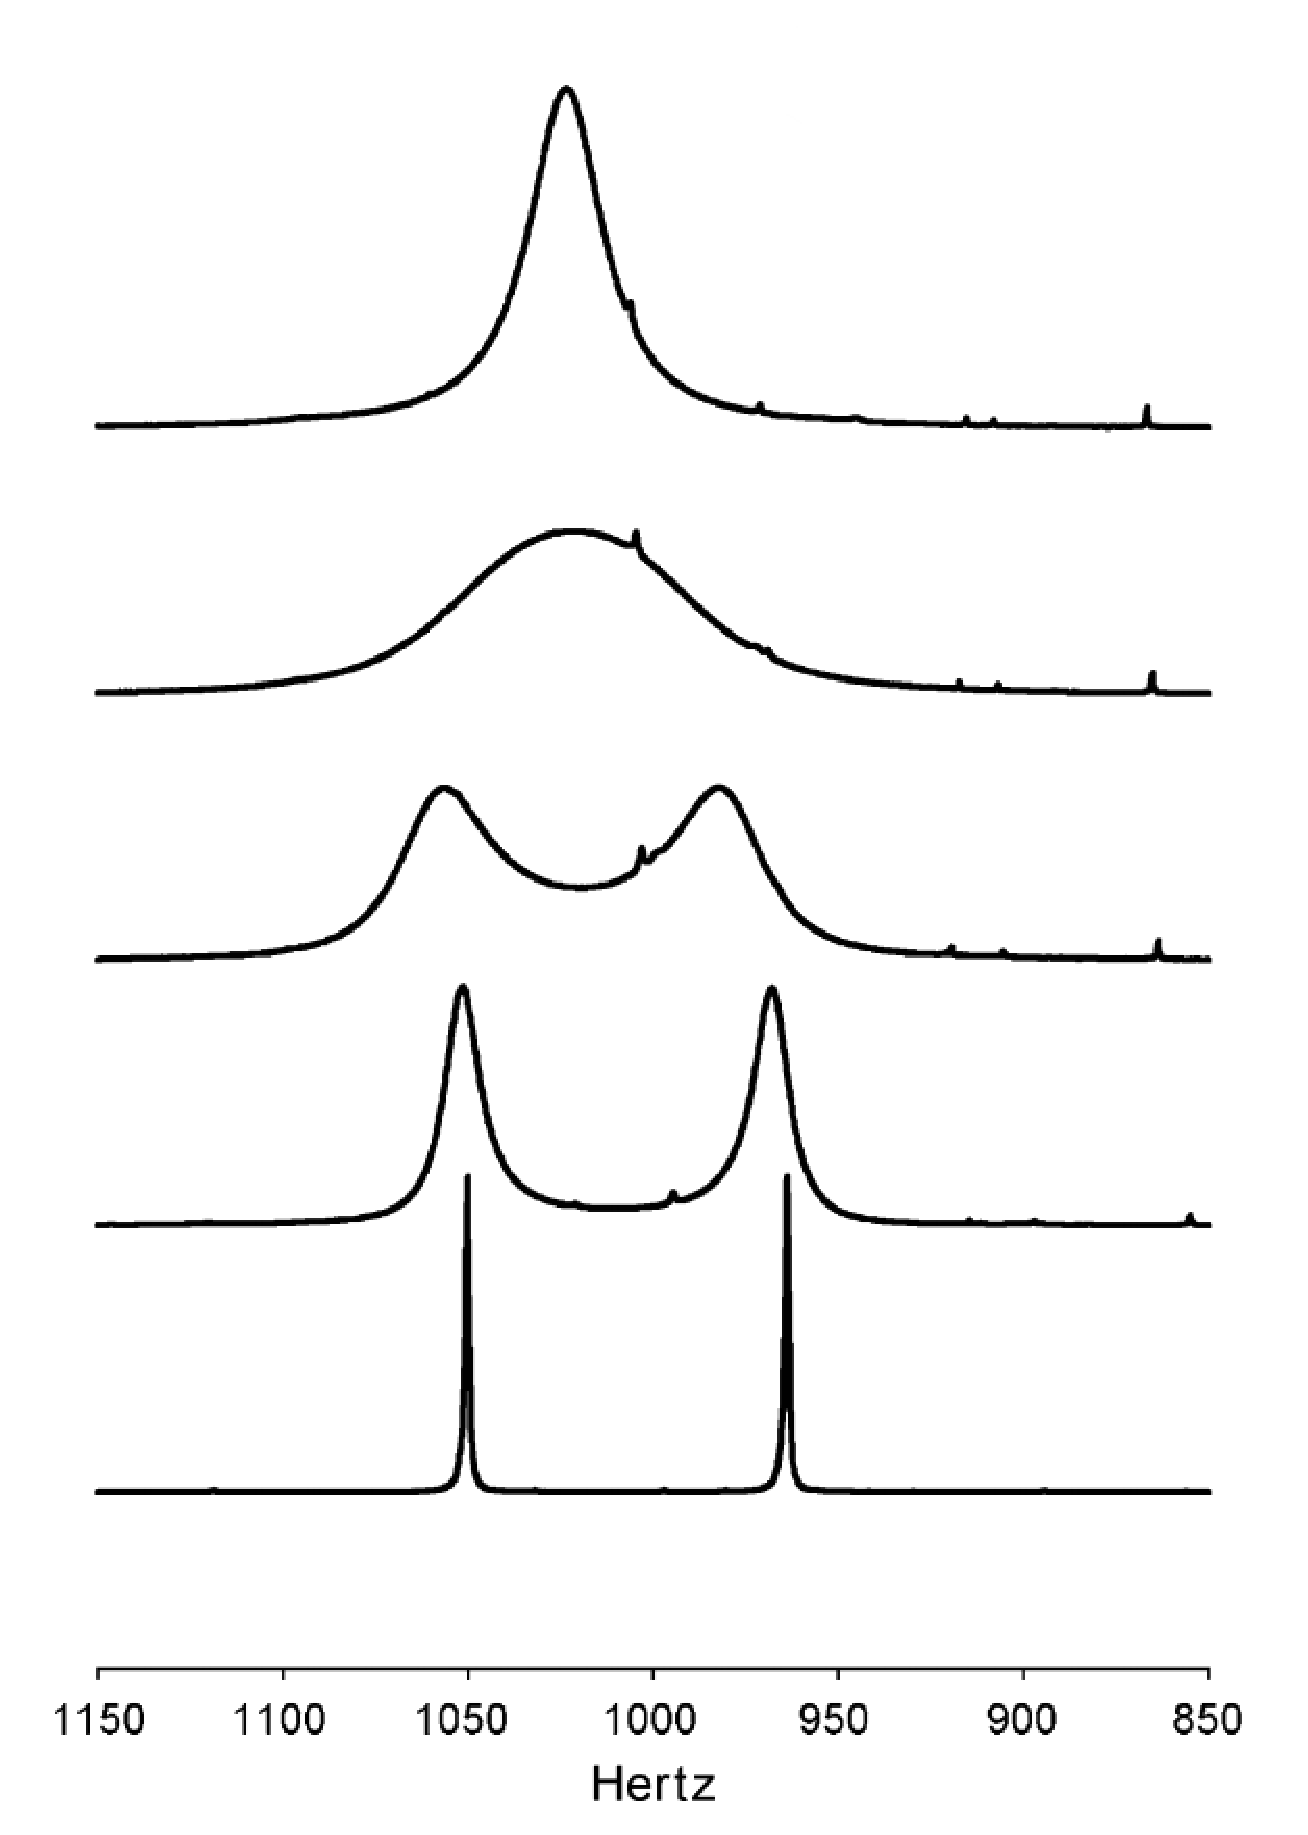
\includegraphics[scale=0.5]{figures/chap2/methyldat.eps}
\caption{"Proton NMR spectra at 300 MHz of the $N$-methyl signals in a
derivative of azapropazone as a function of temperature. The lowest spectrum is at 223 K, and then
at 243, 253, 263, and 273 K"~\cite{Bain200363}}
\label{figure:datamet}
\end{center}
\end{figure}  
Treatment of simple molecular motions and chemical exchange well described in Gamilel ~\cite{gamilel} where they start from determination of absorption spectra by analogy of finding correlation function of classical harmonic oscillator similar to Kubo, Anderson and Blume treatment. Stochastic matrix $W$ introduced in Eq. \ref{eq:34},\ref{eq:35} and \ref{eq:37}that defines transition probability per unit time between stochastic states $a$ and $b$ has the following form:  
For this specific example $p_a=p_b=1/2$. Derivation of proper $W$ matrix and assigning a priori probabilities is a key to correct computation of absorption spectra for complex dynamic environment.Assuming that a priori probabilitieas are equal transition rate is uniform for between the transitions so that $w_{a,b}=w_{b,a}=T$ where $T$ is a transition rate \\*
Time dependent Hamiltonian in Blume\cite{blume} represents nuclear Zeeman interaction and can be constructed as following: 
\begin{equation}\label{eq:58}
\mathcal{H}(t)=\sum_jV_jf_j(t)=B_0I_z+\vec{h}\cdot\hat{I}f(t)
\end{equation}  
Fixed magnetic field $B_0$ by NMR and EPR convention in this case is set along $z$ axis and fluctuating local field $h(x,y,z)$ can point in any arbitrary direction. Stochastic function $f(t)$ can take two values 1 or -1. In feasable form Eq. \ref{eq:58} can be written as: 
\begin{equation}\label{eq:blumeham}
\mathcal{H}(t)=B_0I_z+f(t)\big[\frac{1}{2}(h_+I_-+h_-I_+)+h_zI_z\big]
\end{equation}     
Where $I_{\pm}$ are rising and lowering nuclear spin operators and $h_{\pm}=h_x\pm h_y$ and $h_z$ defines fluctuating field in assosiated with spin operators in $x,y,z$ planes. \\*
Dimension of Liouville matrix is $8\times 8$ and its precise and accurate construction from Eq. \ref{eq:35} is presented in Eq.\ref{eq:60}. In the case when local fluctuating fields aligned with the applied field $h_+=h_-=0$ matrix Eq.\ref{eq:60} reduces to banded or sparse matrix with two non-zero diagonals Eq.\ref{eq:61}. Thus $8\times 8$ matrix reduce to four $2\times 2$ and from computational prospective it is possible to take to account only the two middle matrices and invert them separately which is less time consuming. This is not always the case and in EPR and off-diagonal elements can carry important structural information. \\*
Following procedure from Blume \cite{blume} fixed field was set to $B_0=3$ and fluctuating field $h=h_x=h_y=h_z=4$. Results are presented on Fig.\ref{figure:blumediag}. For all (a), (b) and (c) for fast modulation regime line shape is represented by sharp Lorentizan peak centred around Zeeman frequency. At shorter transition rates thus slow relaxation regime case (a) and (b) represent absorption spectra with fluctuating local fields along $x$ and $y$ axis. The peak roughly occurs at $\omega\approx(B_0^2+h^2)^{1/2}$. Additional Broad side peak at  Fig.\ref{figure:blumediag}(a) can be explained as image of electric non-static Gaussian electron field strength distribution. For the case at Fig.\ref{figure:blumediag}(c) fluctuating field along $z$ axis and two lines correspond to each of the two state frequencies defined as $\omega\approx B_0\pm h$. Fig.\ref{figure:blumediag}(c) corresponds to classical example of temperature dependence of NMR and EPR spectrum due to chemical exchange. In all three cases with the increasing of transition rates lines are broadening at some moderate rate and then collapse into one narrowed line as change of stochastic transitions averages out. \\*
Simulated figures at Fig.\ref{figure:blumediag}(c) completely agrees with originally proposed by Blume \cite{blume} and were obtained by manually typing Liouville matrix and performing inversion and summation to obtain absorption spectra and by AI generalized algorithm. Both computational cases converged to one solution which was an indicator of AI validity and robustness.           
           
\clearpage
\begin{landscape}
\begin{equation}\label{eq:60}
\mathcal{L} = \begin{bmatrix}
       p-w_{aa} & -w_{ab} & \frac{1}{2}h_+ & 0 & -\frac{1}{2}h_- & 0 & 0 & 0  \\[0.3em]
       -w_{ba} & p-w_{bb} & 0 & -\frac{1}{2}h_+ & 0 & \frac{1}{2}h_- & 0 & 0  \\[0.3em]
       \frac{1}{2}h_- & 0 & p-w_{aa}-i(B_0+h_z) & -w_{ab} & 0 & 0 & -\frac{1}{2}h_- & 0  \\[0.3em]
       0 & -\frac{1}{2}h_- & -w_{ba} & p-w_{bb}-i(B_0-h_z) & 0 & 0 & 0 & \frac{1}{2}h_-  \\[0.3em]
       -\frac{1}{2}h_+ & 0 & 0 & 0 & p-w_{aa}-i(B_0+h_z) & -w_{ab} & \frac{1}{2}h_+ & 0  \\[0.3em]
       0 & \frac{1}{2}h_+ & 0 & 0 & -w_{ba} & p-w_{bb}+i(B_0-h_z) & 0 & -\frac{1}{2}h_+  \\[0.3em]
       0 & 0 & -\frac{1}{2}h_+ & 0 & \frac{1}{2}h_- & 0 & p-w_{aa} & -w_{ab}  \\[0.3em]
       0 & 0 & 0 & \frac{1}{2}h_+ & 0 & -\frac{1}{2}h_- & -w_{ba} & p-w_{bb} 
     \end{bmatrix}
\end{equation}
\end{landscape} 

\begin{landscape}
\begin{equation}\label{eq:61}
\mathcal{L} = \begin{bmatrix}
       p-w_{aa} & -w_{ab} & 0 & 0 & 0 & 0 & 0 & 0  \\[0.3em]
       -w_{ba} & p-w_{bb} & 0 & 0 & 0 & 0 & 0 & 0  \\[0.3em]
       0 & 0 & p-w_{aa}-i(B_0+h_z) & -w_{ab} & 0 & 0 & 0 & 0  \\[0.3em]
       0 & 0 & -w_{ba} & p-w_{bb}-i(B_0-h_z) & 0 & 0 & 0 & 0  \\[0.3em]
       0 & 0 & 0 & 0 & p-w_{aa}-i(B_0+h_z) & -w_{ab} & 0 & 0  \\[0.3em]
       0 & 0 & 0 & 0 & -w_{ba} & p-w_{bb}+i(B_0-h_z) & 0 & 0  \\[0.3em]
       0 & 0 & 0 & 0 & 0 & 0 & p-w_{aa} & -w_{ab}  \\[0.3em]
       0 & 0 & 0 & 0 & 0 & 0 & -w_{ba} & p-w_{bb} 
     \end{bmatrix}
\end{equation}
\end{landscape} 

\begin{figure}[h!]
\centering
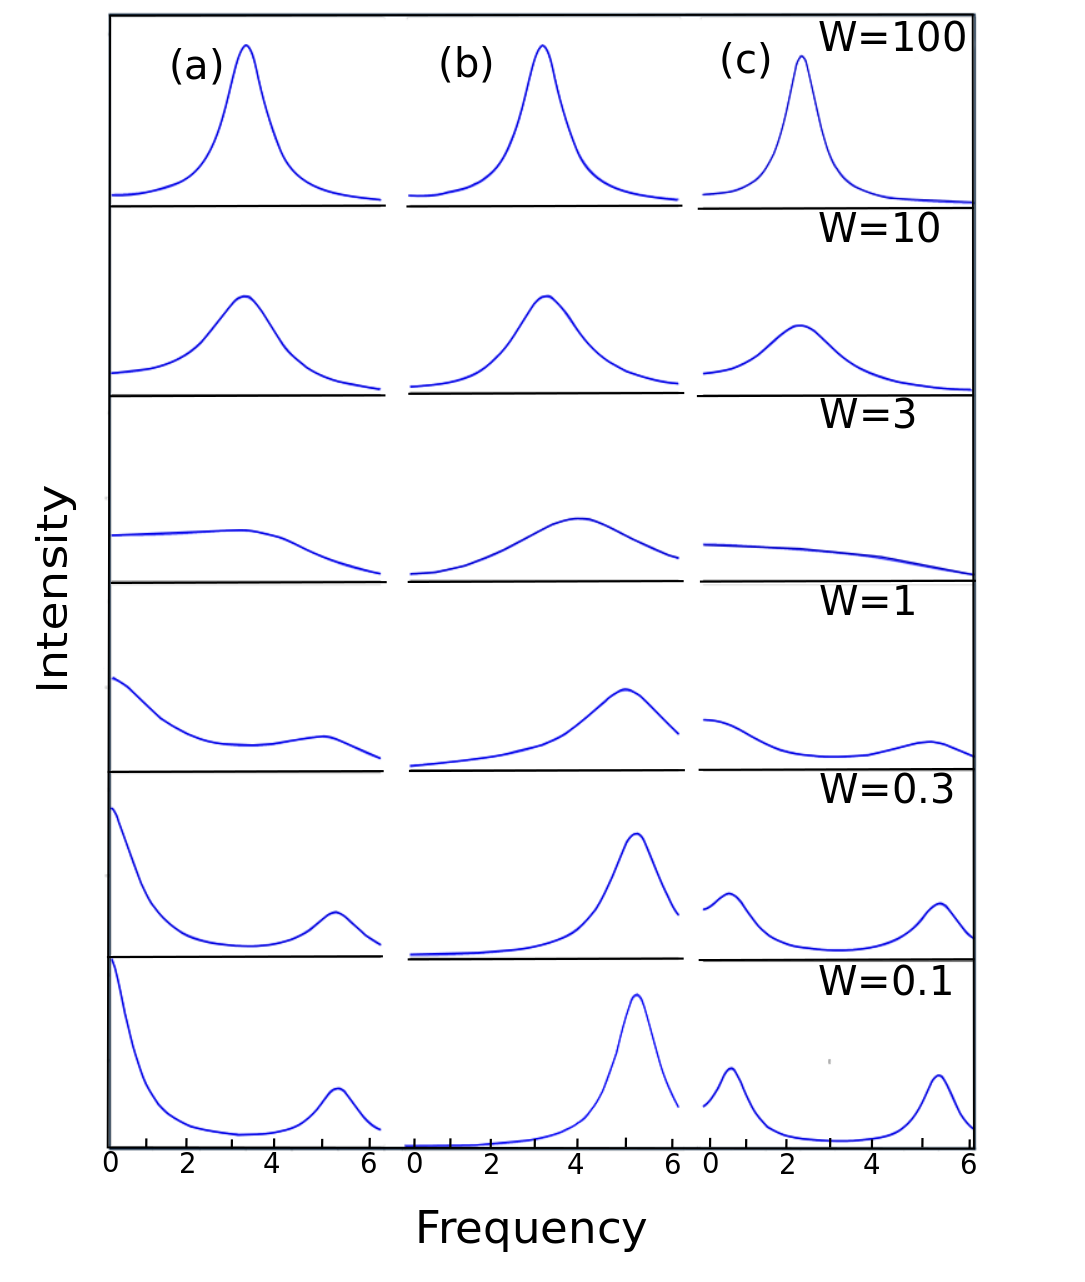
\includegraphics[width=0.7\textwidth]{figures/chap2/blumediag.png}
\caption{Evolution of NMR line shapes with increase of transition rates $W$ for $I=1/2$ nucleus in a fixed magnetic field along $z$ axis and fluctuating local magnetic fields $h$ along (a) $x$ axis, (b) $y$ axis and (c) $z$ axis. Simulated using AI alagorithm}
\label{figure:blumediag}
\end{figure}
\clearpage
\subsection{Anisotropic Zeeman}\label{zeemansection}
To examine if the model is valid for axial asymmetric contributing terms of Hamiltonian first proper construction inculding orientation dependence should be made. Effective anisotropic Hamiltonian for isolated unpaired electron in tensor contraction form using Eq.\ref{eq:58} and Eq.\ref{eq:60} with $g$-tensor components transformed into the laboratory frame\cite{NMRtomograph}\cite{Nordio} using Eq.\ref{eq:47}:
\begin{subequations}\label{eq:48}
\begin{align}
A^{[2],L}_{\pm2,(g)} & =-\frac{1}{2}S_{\pm}B_{\pm}\\
A^{[2],L}_{\pm1,(g)} & =\pm\frac{1}{2}(S_{\pm}B_{z}+S_zB_{\pm})\\
A^{[2],L}_{0,(g)} & =-\sqrt{\frac{2}{3}}\big(S_{z}B_{z}-\frac{1}{4}(S_+B_-+S_-B_+)\big)\\
A^{[0],L}_{0,(g)} & =\frac{1}{\sqrt{3}}\big(S_{z}B_{z}+\frac{1}{2}(S_+B_-+S_-B_+)\big)
\end{align}
\end{subequations}
Where $B_{\pm}=B_x\pm iH_y$. Choosing applied magnetic filed being oriented along $z$ axis in the laboratory frame  Eq.\ref{47}a and Eq.\ref{eq:47}b are vanishing: 
\begin{subequations}\label{eq:49}
\begin{align}
A^{[2],L}_{\pm2,(g)} & =0\\
A^{[2],L}_{\pm1,(g)} & =0\\
A^{[2],L}_{0,(g)} & =-\sqrt{\frac{2}{3}}S_{z}B_{z}\\
A^{[0],L}_{0,(g)} & = \frac{1}{\sqrt{3}}(S_{z}B_{z}
\end{align}
\end{subequations}
The $g$-tensor decompose into rank-zero tensor $g^{(0,0)}$ and five components of second-rank tensor $g^{(2,m)}\rightarrow(g^{(2,\pm2)}, g^{(2,\pm1)},g^{(2,0)})$. Writing in principal axis frame IST components are: 
\begin{subequations}\label{eq:50}
\begin{align}
F^{[2],P}_{\pm2,(g)} & =-\frac{1}{2}\beta_e(g_{xx}-g_{yy})\\
F^{[2],P}_{\pm1,(g)} & =0\\
F^{[2],P}_{0,(g)} & =-\sqrt{\frac{2}{3}}\beta_e\big(g_{zz}-\frac{1}{2}(g_{xx}-g_{yy})\big)\\
F^{[0],P}_{0,(g)} & = \frac{1}{\sqrt{3}}\beta_e(g_{xx}+g_{yy}+g_{zz})
\end{align}
\end{subequations}
From the definition:
\begin{equation}
F^{[2],L}_{m,g}=\sum_{m'}(-1)^m(\mathcal{D}^{[2]}_{m,m'}(\alpha,\beta,\gamma))^*F^{[2],P}_{m',g}
\end{equation}
And using Wigner matrix elements from Tab.\ref{tab:wigner} in simple form:  
\begin{multline}\label{eq:tensorzeem}
F^{[2],L}_{m,g}=(-1)^m\Big(\big(\mathcal{D}^{[2]}_{m,2}(\alpha,\beta,\gamma)+\mathcal{D}^{[2]}_{m,-2}(\alpha,\beta,\gamma))F^{[2],P}_{2,g}+\mathcal{D}^{[2]}_{m,0}(\alpha,\beta,\gamma)F^{[2],P}_{0,g}\Big)= \\ =(-1)^m\Big((e^{im\alpha}d_{-m,2}^2(\beta)e^{-i2\gamma}+e^{im\alpha}d_{-m,2}^2(\beta)e^{i2\gamma}) F^{[2],P}_{2,g}+e^{im\alpha}d_{-m,0}^2(\beta)F^{[2],P}_{0,g}\Big)
\end{multline}
And finally in terms of matrix elements for $m=-2...2$
\begin{subequations}\label{eq:dmatel}
\begin{align}
F^{[2],L}_{-2,g}& = e^{-i2\alpha}\Big[(\frac{1+\cos^2\beta}{2}\cos2\gamma-i\cos\beta\sin2\gamma) F^{[2],P}_{2,g}+\sqrt\frac{3}{8}\sin^2\beta F^{[2],P}_{0,g} \Big]\\
F^{[2],L}_{-1,g}& = -e^{-i\alpha}\Big[(\cos\beta\cos\beta\cos2\gamma-i\sin\beta\sin2\gamma) F^{[2],P}_{2,g}+\sqrt\frac{3}{2}\sin\beta\cos\beta F^{[2],P}_{0,g} \Big]\\
F^{[2],L}_{0,g}& = \sqrt\frac{3}{2}\sin^2\beta\cos2\gamma F^{[2],P}_{2,g}+\frac{1}{2}(3\cos^2\beta-1)F^{[2],P}_{0,g} \\
F^{[2],L}_{1,g}& = e^{i\alpha}\Big[(\cos\beta\cos\beta\cos2\gamma+i\sin\beta\sin2\gamma) F^{[2],P}_{2,g}+\sqrt\frac{3}{2}\sin\beta\cos\beta F^{[2],P}_{0,g} \Big]=(F^{[2],L}_{2,g})^*\\
F^{[2],L}_{2,g}& = e^{i2\alpha}\Big[(\frac{1+\cos^2\beta}{2}\cos2\gamma+i\cos\beta\sin2\gamma) F^{[2],P}_{2,g}+\sqrt\frac{3}{8}\sin^2\beta F^{[2],P}_{0,g} \Big]=(F^{[2],L}_{2,g})^*
\end{align}
\end{subequations}
To summarize the Hamiltonian in the comlicated case for assymetric $g$-tensor including both "secular" and "non-secular" terms: 
\begin{equation}
\mathcal{H}_{eff}=A_0^{[0]}F_0^{[0]}+A_0^{[2]} F_0^{[2]}+A_{+2}^{[2]} F_{+2}^{[2]}+A_{-2}^{[2]} F_{-2}^{[2]}
\end{equation}
For non-saturated lines it is enough to include only "secular" part which is the interaction term proportional to $S_z$ operator bounding states to themselves. It is true if correlation time is short compared to inverse of the Larmor frequency. 
\begin{equation}
\mathcal{H}_{eff}=(\frac{1}{\sqrt{3}}S_zB_z)F_0^{[0]}+(-\sqrt\frac{2}{3}S_zB_z)F_0^{[2]}
\end{equation}
Simulated spectra for anisotropic $g$-tensor contribution with rhombic axial symmetry is presented on figure ~\ref{figure:gten1}. Spectra is extremely sensitive to the adjusting parameters of the model as well as transition rates. For example effect of rhombic symmetry is observable for the rates lower then $0.05$othervise the one Lorentzian peak is observed. Resolution should be set no lower then 0.01 othervise the same Lorentzian line shape is presented. 
\begin{figure}[h!]
\centering
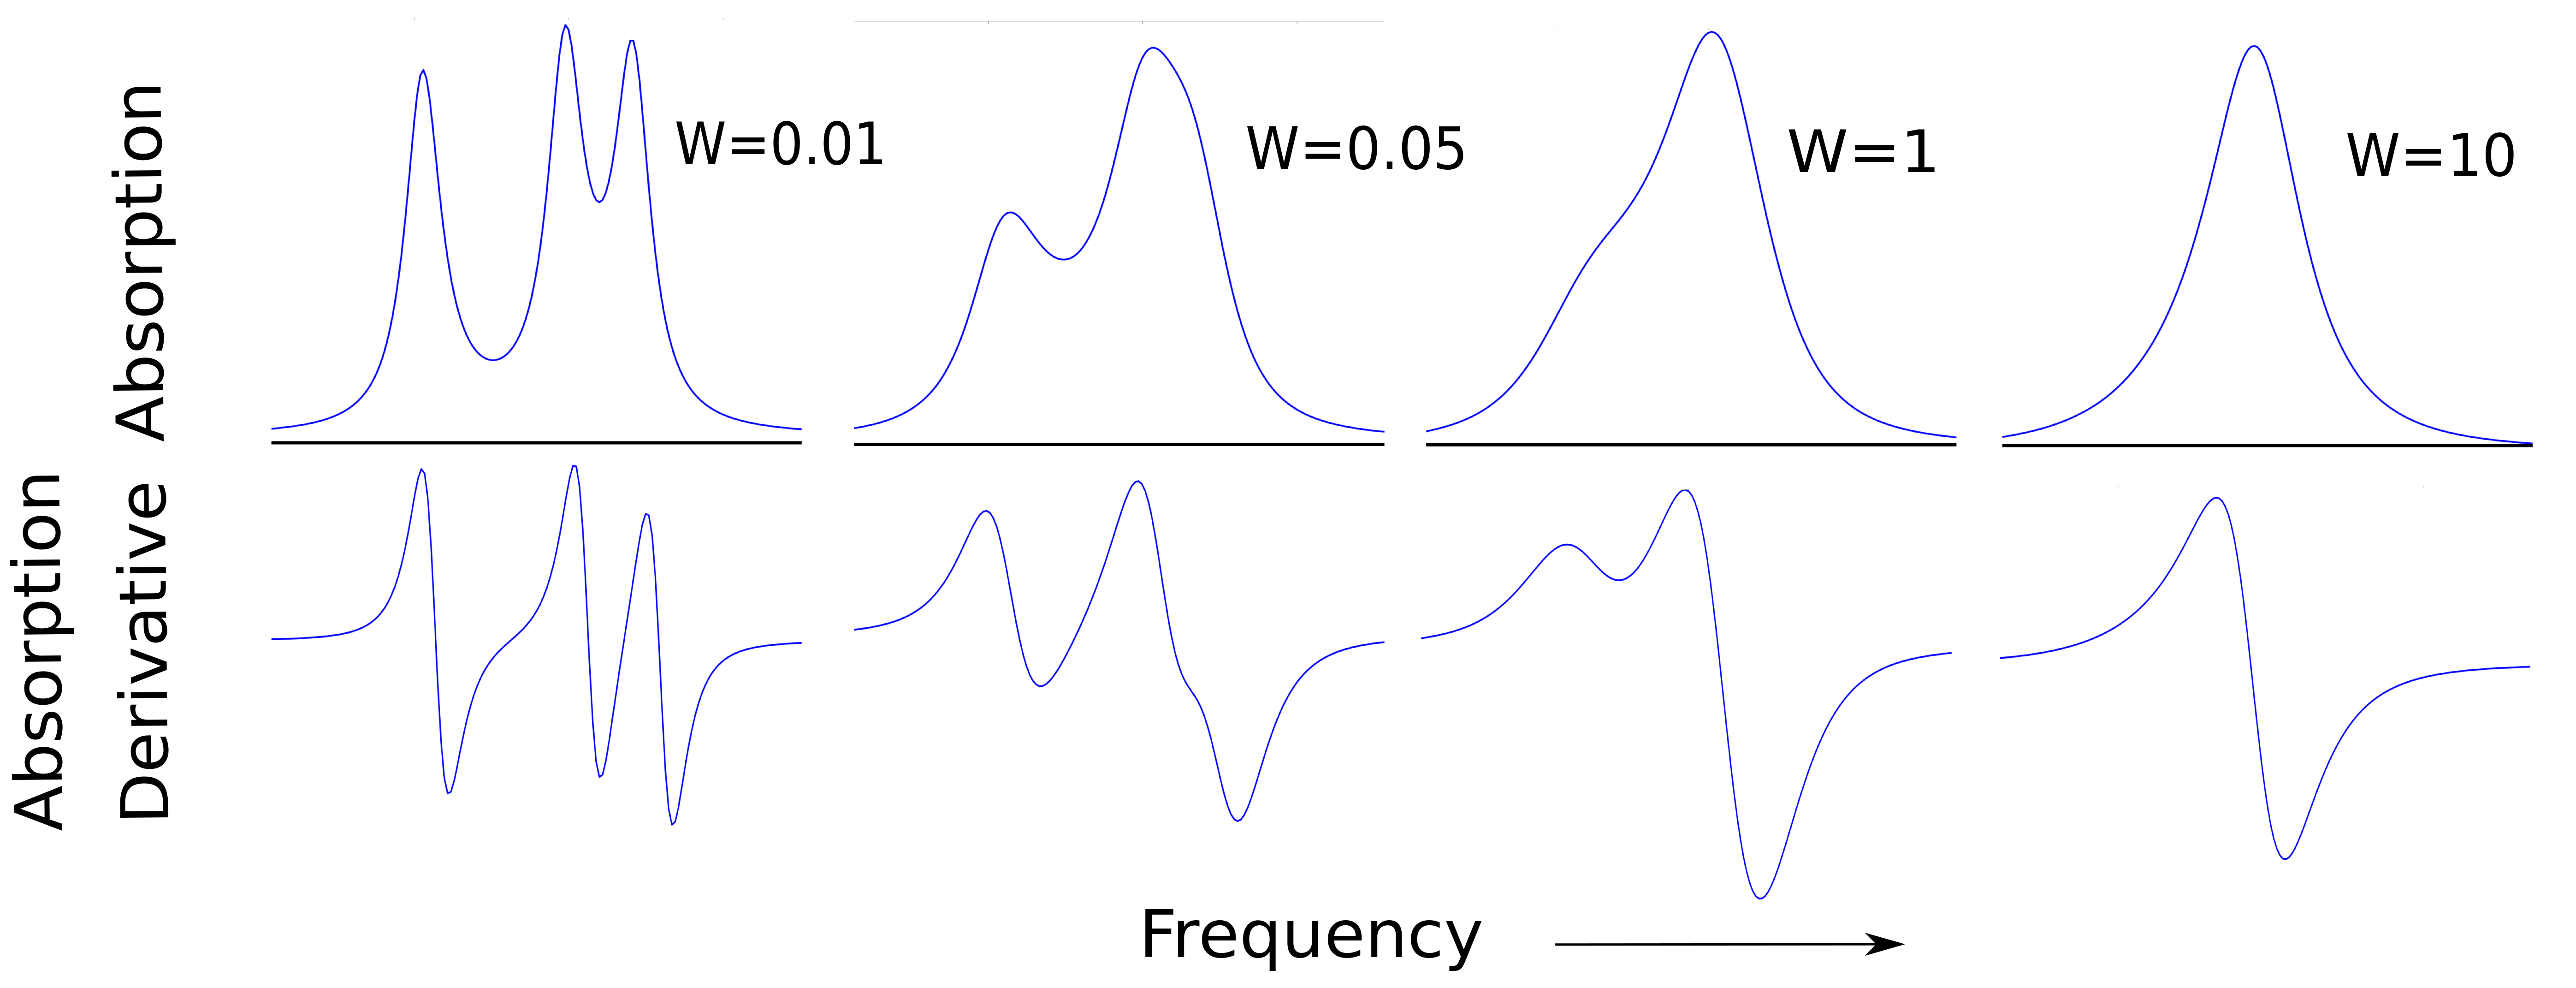
\includegraphics[height=8cm,width=1\textwidth]{figures/chap2/gtenanisat1.png}
\caption{Evolution of NMR line shapes with increase of transition rates $W$ for $I=1/2$ nucleus in a fixed magnetic field along $z$ axis and fluctuating local magnetic fields $h$ along (a) $x$ axis, (b) $y$ axis and (c) $z$ axis. Simulated using AI alagorithm}
\label{figure:gten1}
\end{figure}
There are no significant differences between 6 and 48 stochastic brining computational relief to us. 
\begin{figure}[h!]
\centering
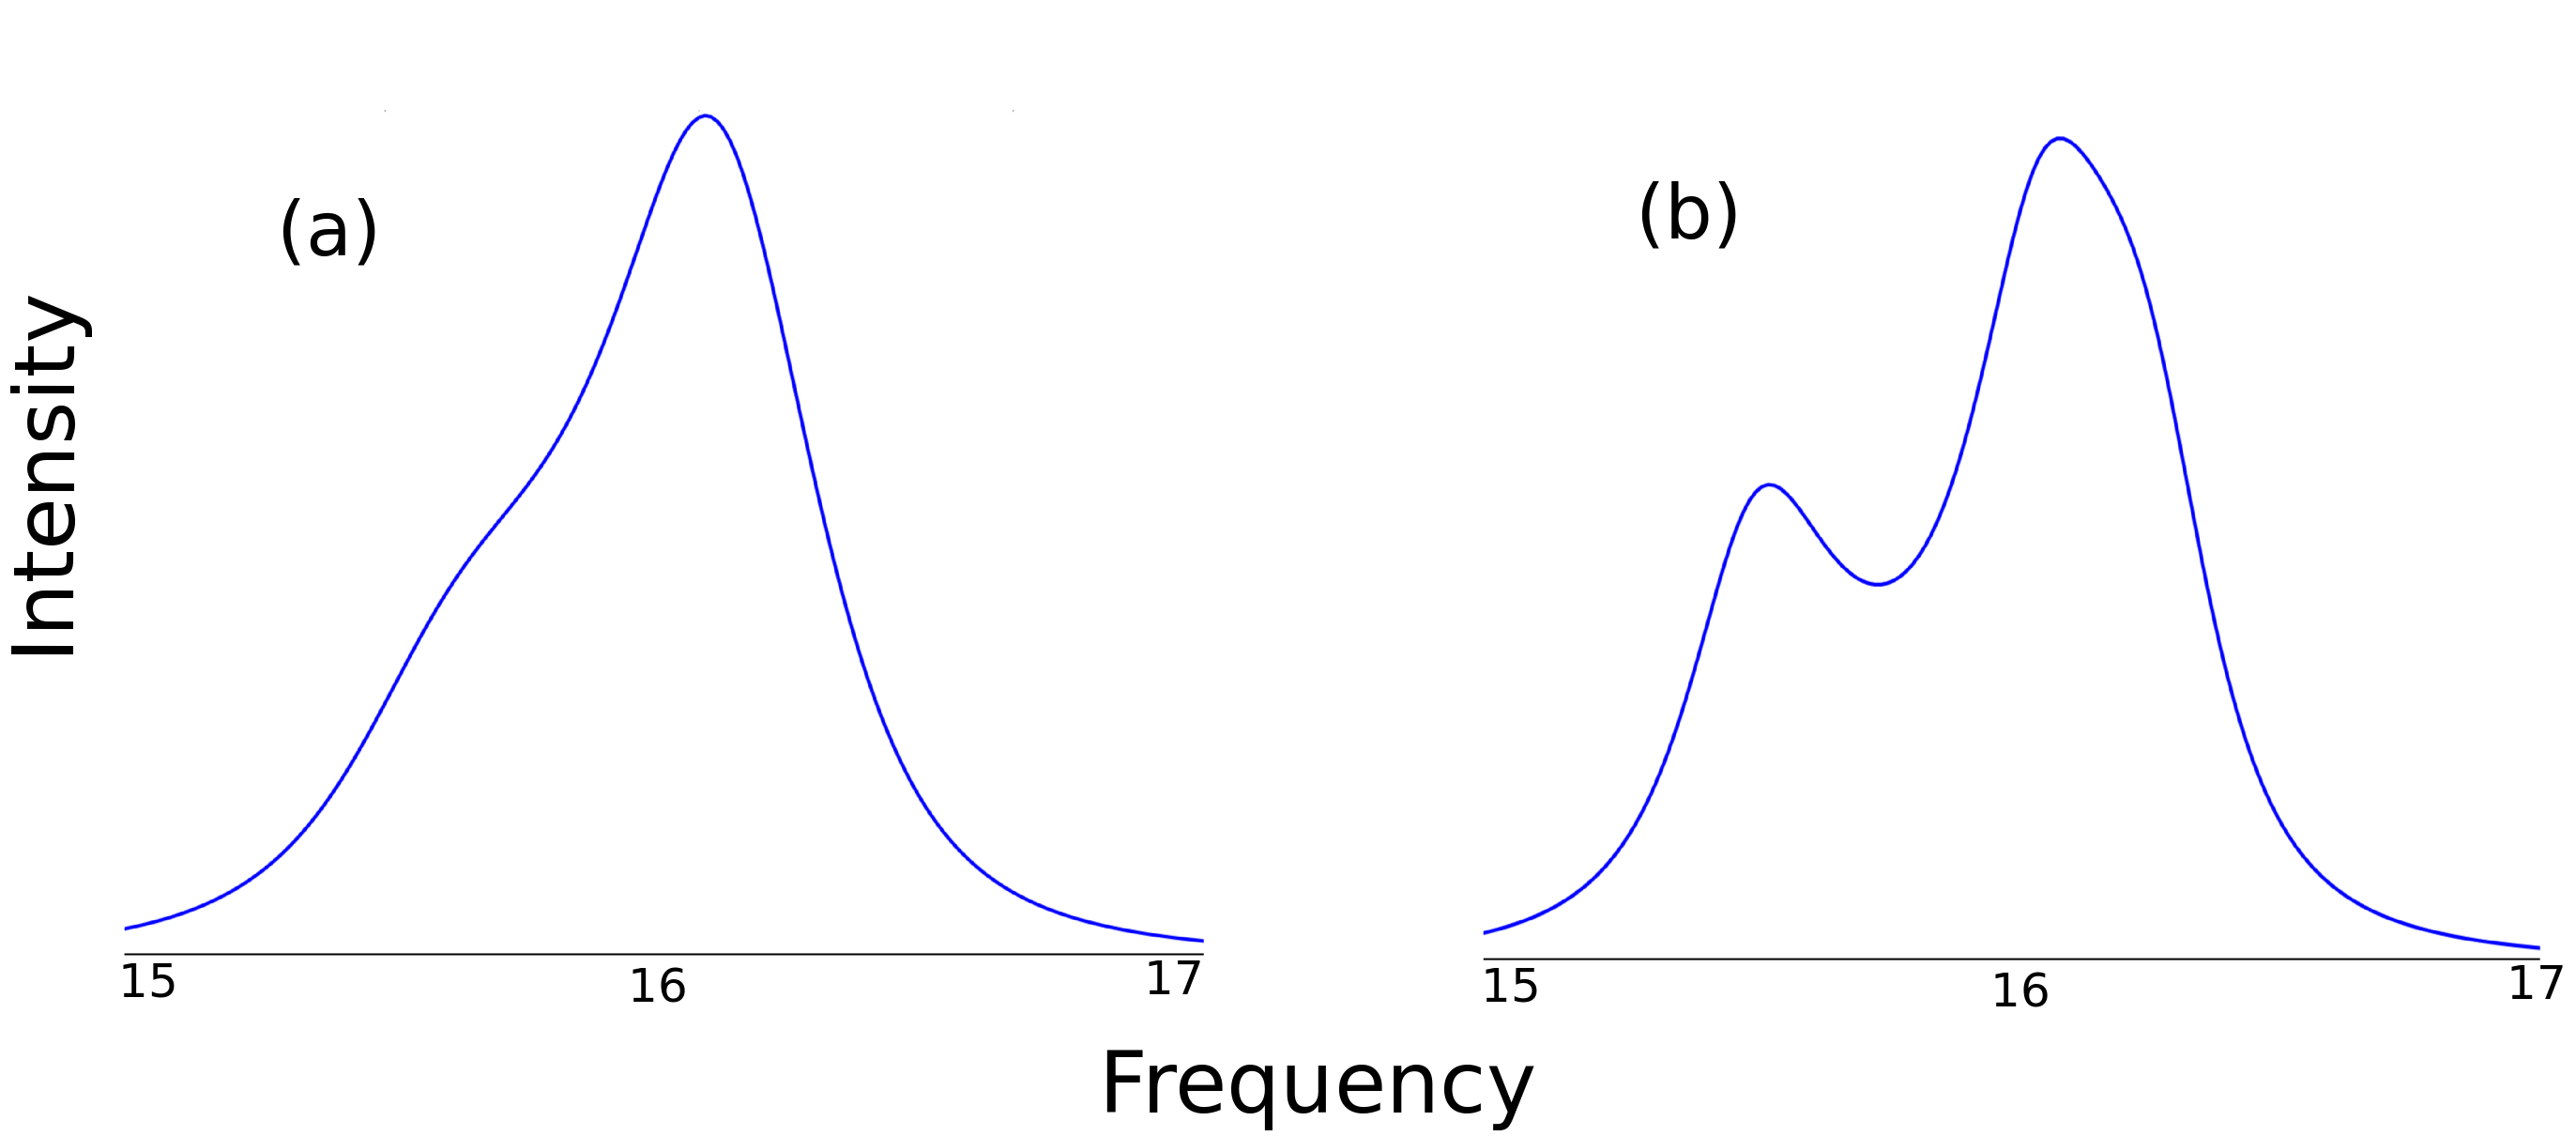
\includegraphics[height=8cm,width=1\textwidth]{figures/chap2/gtenanisat2.png}
\caption{Evolution of NMR line shapes with increase of transition rates $W$ for $I=1/2$ nucleus in a fixed magnetic field along $z$ axis and fluctuating local magnetic fields $h$ along (a) $x$ axis, (b) $y$ axis and (c) $z$ axis. Simulated using AI alagorithm}
Interestingly that using unequal a priori probability between states transition and using transition rates matrix designed in Eq.\ref{eq:Wmat2} setting $s=0.1,m=1$ and $f=100$ line shape tend to represent the case of axial symmetry or that $g_{xx}=g_{yy}<g_{zz}$ 
\label{figure:gterates}
\end{figure}
\clearpage
\subsection{Coupled Spins 1/2}\label{05coupledspinsection}
The more complicated and fascinating interest for our group occurs when unpaired electron spin is interacting with nuclei. Thus a hyperfine interaction should be added. But first lets modify Eq.\ref{eq:37} adding additional sets of bra and kets for the unpaired electron quantum states $\langle m_{0s},m_{1s},S_0,S_1|$ and $|S_0,S_1,m_{0s}',m_{1s}'\rangle$ on both sides.  
\begin{multline}\label{eq:newbras}
P(\omega)=
\frac{2}{\Gamma(2I_0+1)}\mathcal{H}^{(-)}\delta_{m_{1I}m_{0I}}\delta_{m_{1S}m_{0S}}\mathcal{H}^{(+)}\delta_{m_{1I}'m_{0I}'}\delta_{m_{1S}'m_{0S}'} \\ \times[s\delta_{ab}\delta_{m_{1I}m_{1I}'}\delta_{m_{0I}m_{0I}'}\delta_{m_{1S}m_{1S}'}\delta_{m_{0S}m_{0S}'}-(a|W|b)\delta_{m_{0I}m_{0I}'}\delta_{m_{1I}m_{1I}'}\delta_{m_{0S}m_{0S}'}\delta_{m_{1S}m_{1S}'} \\ -i(a|F|a)\delta_{ab}[\langle I_0S_0m_{0I}m_{0S}|V_j|I_0S_0m_{0I}'m_{0S}'\rangle \delta_{m_{0I}m_{0I}'}\delta_{m_{0S}m_{0S}'}\\-\langle I_1S_1m_{1I}m_{1S}|V_j|I_1S_1m_{1I}'m_{1S}\rangle\delta_{m_{1I}m_{1I}'}\delta_{m_{1S}m_{1S}'}]^{-1}
\end{multline} 
Starting vectors $\mathcal{H}^{(+)}$ and $\mathcal{H}^{(-)}$ that define proper electronic magnetization components for the line shape are modified accordingly to \cite{bmr}: 
\begin{equation}
\langle \mathcal{H}^{(+)} \rangle=\langle S_x\otimes I_1 \rangle
\end{equation}
Where $I_1$ is a unit operator in nuclear spin space. $\langle S_x\rangle$ can be easily found in terms of rising and lowering operators and corresponding matrix constructed. \\*
Similarly to the ISTO transformation of the Zeeman part of Hamiltonian it is possible to write all components of the transformed hyperfine interaction term. Starting with spin operators in laboratory frame:   
\begin{subequations}\label{eq:hyperA}
\begin{align}
A^{[2],L}_{\pm2,(hf)} & =-\frac{1}{2}S_{\pm}I_{\pm}\\
A^{[2],L}_{\pm1,(hf)} & =\pm\frac{1}{2}(S_{\pm}I_{z}+S_zI_{\pm})\\
A^{[2],L}_{0,(hf)} & =-\sqrt{\frac{2}{3}}\big(S_{z}I_{z}-\frac{1}{4}(S_+I_-+S_-I_+)\big)\\
A^{[0],L}_{0,(hf)} & =\frac{1}{\sqrt{3}}\big(S_{z}I_{z}+\frac{1}{2}(S_+I_-+S_-I_+)\big)
\end{align}
\end{subequations}
Correspondingly principal components of the $A$-tensor: 
\begin{subequations}\label{eq:HyperAA}
\begin{align}
F^{[2],P}_{\pm2,(hf)} & =-\frac{1}{2}\beta_e(A_{xx}-A_{yy})\\
F^{[2],P}_{\pm1,(hf)} & =0\\
F^{[2],P}_{0,(hf)} & =-\sqrt{\frac{2}{3}}\beta_e\big(A_{zz}-\frac{1}{2}(A_{xx}+A_{yy})\big)\\
F^{[0],P}_{0,(hf)} & = \frac{1}{\sqrt{3}}\beta_e(A_{xx}+A_{yy}+A_{zz})
\end{align}
\end{subequations}
Transformation between laboratory and principal axis system for the hyperfine interaction can be done in similar fashion as for the $g$ tensor. Working in the linear response regime only commuting terms with the Zeeman Hamiltonian are of interest or in other words terms that are proportional to $S_z$. Effective Hamiltonian for Hyperfine part only can be written thus as: 
\begin{equation}
\mathcal{H}_{eff}'=A_{0,(hf)}^{[0]}F_{0,(hf)}^{[0]}+A_{0,(hf)}^{[2]} F_{0,(hf)}^{[2]}+A_{+1,(hf)}^{[2]} F_{+1,(hf)}^{[2]}+A_{-1,(hf)}^{[2]} F_{-1,(hf)}^{[2]}
\end{equation}
\begin{equation}
\mathcal{H}_{eff}'=(\frac{1}{\sqrt{3}})S_zI_zF_{0,(hf)}^{[0]}+(-\sqrt{\frac{2}{3}})S_zI_zF_{0,(hf)}^{[2]}+\frac{1}{2}S_zI_- F_{+1,(hf)}^{[2]}+(\frac{1}{2})S_zI_+ F_{-1,(hf)}^{[2]}
\end{equation}
The only interest brings the terms that a partially commute with the Zeeman interaction namely that are proportional to $I_z$ operators coupled with $S_z$ or in other words $S_zI_z$. In this way only similar to Zeeman term quantum states are coupled. In the case when hyperfine interaction is strong compared to Zeeman it is important to include a spin "flipping" terms that do not change electronic spin states or terms that are $S_zI_{\pm}$. This terms do not commute with the Zeeman Hamiltonian and they induce additional transition between the sates in the system known as "Pseudosecular". Thus we have approached Blume~\cite{blume} model with the general form of the Hamiltonian. As usual "Nonsecular" terms have been dropped of namely $A_{\pm2,(hf)}^{[2]}$. Now total Hamiltonian assuming that principal component of the Zeeman $g$ tensor and Hyperfine $A$ tensor are coincide so that there are no mutual difference between rotational transformation of their principal components can be written,
\begin{multline}
\mathcal{H}_{total}=H_{eff}+H_{eff}'=\frac{1}{\sqrt{3}}F_{0}^{[0]}(S_zI_z+S_zB_z) \\ +(-\sqrt{\frac{2}{3}})F_{0}^{[2]}(S_zB_z+S_zI_z)+\frac{1}{2}S_zI_- F_{+1}^{[2]} +(\frac{1}{2})S_zI_+ F_{-1}^{[2]}
\end{multline}
To start out with lets consider $S=1/2$ and $I=1/2$ case. Allowed transitions are obvious for the Zeeman interaction and overlapping Hyperfine are defined with the kronecker deltas and more interesting are the two allowed transitions for the "pseudosecular" part of the Hamiltonian:
$$|m_S=-1/2,m_I=1/2\rangle\rightarrow|m_S=1/2,m_I=1/2\rangle$$ 
and 
$$|m_S=-1/2,m_I=-1/2\rangle\rightarrow|m_S=1/2,m_I=-1/2\rangle$$ 
On the Fig.\ref{figure:spin05} result is given including only terms that are commuting with the Zeeman Hamiltonian. 
\begin{figure}[h!]
\centering
\includegraphics[width=1\textwidth]{figures/chap2/gtenanisatotal.eps}
\caption{Evolution of NMR line shapes with increase of transition rates $W$ for $I=1/2$ nucleus in a fixed magnetic field along $z$ axis and fluctuating local magnetic fields $h$ along (a) $x$ axis, (b) $y$ axis and (c) $z$ axis. Simulated using AI alagorithm}
\label{figure:spin05}
\end{figure}
\begin{figure}[h!]
\centering
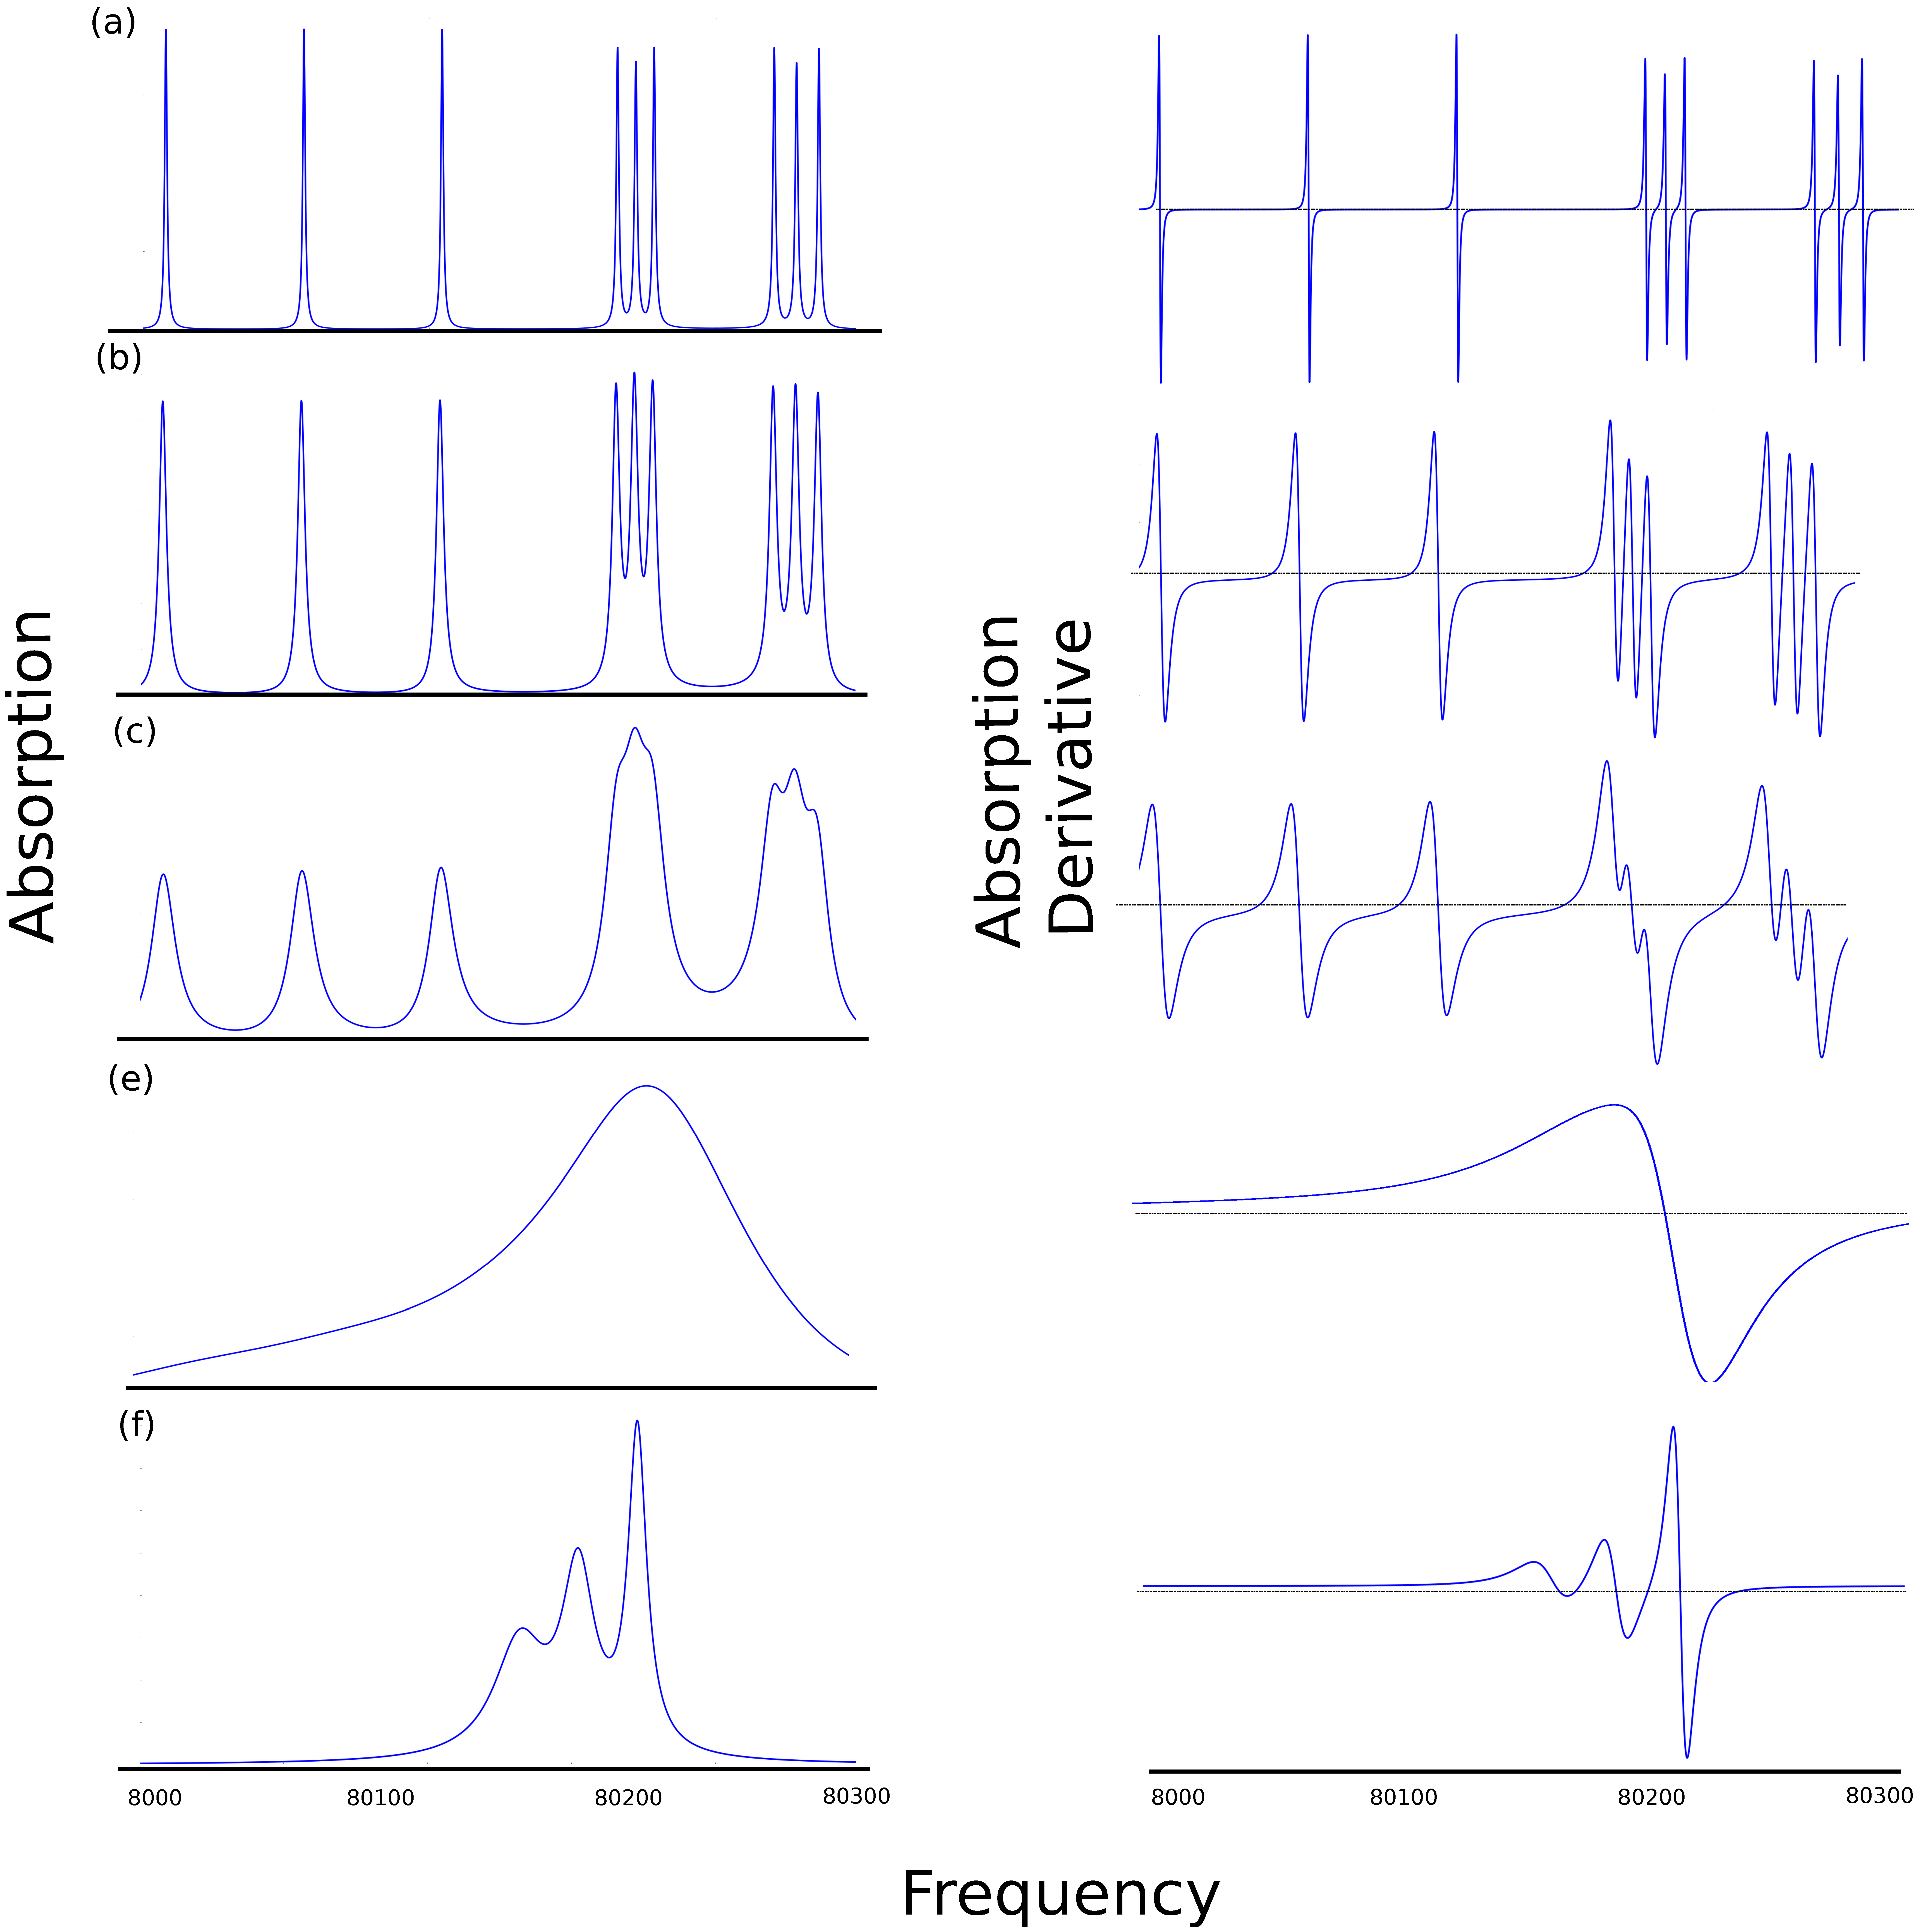
\includegraphics[width=1\textwidth]{figures/chap2/spinone.eps}
\caption{Evolution of NMR line shapes with increase of transition rates $W$ for $I=1/2$ nucleus in a fixed magnetic field along $z$ axis and fluctuating local magnetic fields $h$ along (a) $x$ axis, (b) $y$ axis and (c) $z$ axis. Simulated using AI alagorithm}
\label{figure:spin05der}
\end{figure}
\clearpage
%\chapter{Applied Machine Learning for classification problems in Chemistry}
\section{Introduction}
Like in magnetic resonance, majority of early developed models such as first description of perceptron or simple neuron were done by McCulloh and Pitts in 1943\cite{McCulloch1943} but were not used due to the lack of computational power. With rise of distributed computing specifically in this decade field of Artificial Intelligence gain a significan boost with Graphical Processing Unit (GPU) computations decreasing in some cases training of extensive machine learning models from monthes to simply hours with minimum cost involved. This simply greatly impacted variety of applications of ML to solve actual real world problems such as fracture detection from X-ray images\cite{Tian2003} or cancer prediction using gene expression profiling\cite{khan:2001}. Machine Learning models are divided in two groups: Supervised and Unsupervised. Supervised models are such models that require labled data from which they "learn" data in order to be able predict label for the newly introduced data. Typicaly this are Arificial Neural Networks, Support Vector Machines and etc. Unsupervised models are trying to gather insight from the data and group it accordingly to self-defined class or labels, intuitively this are clustering models such as hierrarhical or k-means algorithms. Widely for some problems unsupervised models are used fo prprocessing to perform demensionality reduction in order to fight curse of dimensionality, when extra-features can reduce greatly the predictive power. In this work we will specifically work with supervised models and some unsupervised algortihms were used for geature selection. In this chpater we will discuss how one can use Support Vector Machines, Arificial Neural Networks, Genetic Algorithms and their limitations. We will also discussed bottlenecks that we have faced during this work such as overfitting after preprocessing and etc. 
\subsection{Support vector Machines}
Support Vector Machines(SVMs) is a really well known and used supervised machine learning technique for data classification. It was first developed by Vladimir Vapnik an soviet expatriate to United States who worked at that time for AT\& T Bell Labs. In a simply few words idea of SVMs is to linearly separate the data which might be non-linearly separable. I will touch main aspects of theoretical derivation to understand the idea behind SVM and will not dive into mathematical madness.
Lets assume that $X$ is a feature space or space of an objects, and $Y$ is a set of solutions. It is obvious that an algorithm that will find approximate dependencies between the feature $X$-space and the solution $Y$-space have to be found in form $F:X\rightarrow Y$.  At the moment lets only deal with binary classification    namely $Y=(-1,+1)$ and feature space is described by $n$-dimensional real vectors $X=\mathbf{R}^n$. 
The classifier will have the form: 
\begin{equation}\label{eq:svm}
F(x)=sign(\sum_{j=1}^{n} \omega_j x_j-\omega_0)=sign(x^{T}\omega-w_0)
\end{equation}
Where $x=(x_1,....,x_n)$- evidential description of an object $X$ whose transpose should be taken; vector $\omega=(\omega_1,....,\omega_n)$ and value of $\omega_0$ are some parameters of the algorithm. And sign of the sum will define to which class corresponds the given feature. If sign is negative solution is $Y=-1$ and if it returns positive $Y=1$. Taking away $sign$ Eq.\ref{eq:svm} defines a hyperplane which has 2 dimensions in a 3-D space and 1-D in a 2-D space. The idea is to generate family of hyperplanes until one that creates biggest margin between training points is found. That means appropriate $\omega$ and $\omega_0$ have to be determined for the specific data set. An example of is give on Fig.\ref{figure:svm1}    
\begin{figure}[h!]
\centering
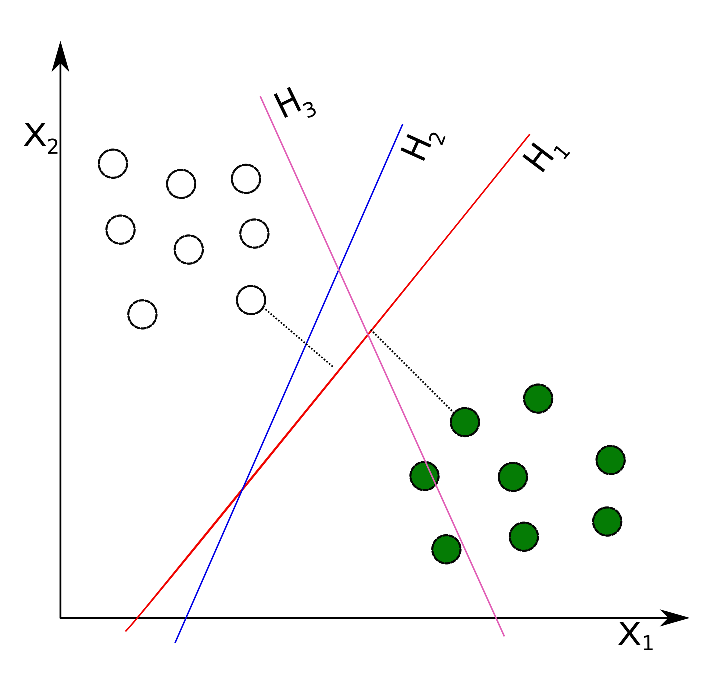
\includegraphics[width=1\textwidth]{figures/chap3/svm1.eps}
\caption{}
\label{figure:svm1}
\end{figure}
If we assume that data set is linearly separable one can define an error function of training as: 
\begin{equation}
Q(\omega,\omega_0)=\sum_{i=1}^l[y_i(\langle \omega,x_i\rangle-\omega_0)<0]
\end{equation}
Conditions on the border: 
\begin{equation}\label{eq:svmb1}
\omega,x_i\rangle-\omega_0=y_i
\end{equation} 
and 
\begin{equation}\label{eq:svmb2}
\langle \omega,x_i\rangle-\omega_0 = \begin{cases} \leq-1, & \mbox{if } y_i=-1 \\ \geq1 , & \mbox{if } y_i=1 \end{cases}
\end{equation}
From Eq.\ref{eq:svmb1} and Eq.\ref{eq:svmb2} it is obvious that hyperplane should be tied by the condition: 
\begin{equation}\label{eq:svmb3}
-1<\langle \omega,x\rangle-\omega_0<1
\end{equation}
It is pretty obvious that separation width between to classes can be defined as $\frac{2}{||\omega||}$ and it is more clear on Fig.\ref{figure:svm2}.  
\begin{figure}[h!]
\centering
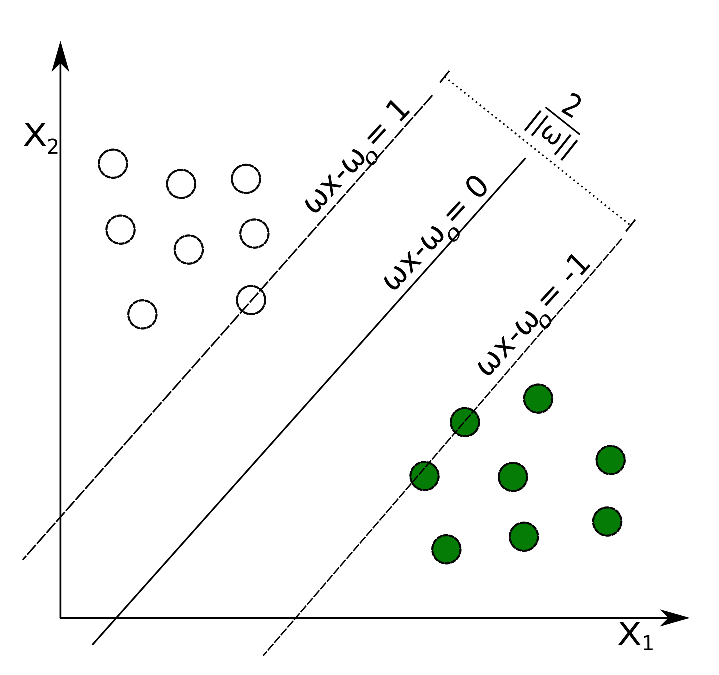
\includegraphics[width=1\textwidth]{figures/chap3/svm2.eps}
\caption{}
\label{figure:svm2}
\end{figure}
If data is perfectly linearly separable then $||\omega||^2$ can be minimized by two constraints: 
\begin{equation}
\begin{cases} \langle \omega,\omega\rangle \rightarrow min;\\ y_i(\langle \omega,x_i\rangle-\omega_0)\geq1 , &  y=1,...,l  \end{cases}
\end{equation}
In more compact form:
\begin{equation}\label{eq:svmconst}
y_i(\omega\cdot x_i+\omega_0)\geq 1
\end{equation}
If features of two classes are allowed to overlap and no longer linear separability is presented it is possible to allow some points to appear on the other or wrong side of margin and to add slack variables such as $\xi=(\xi_1,\xi_2,...,\xi_N)$ or thus constraint from Eq.\ref{eq:svmconst} can be written as: 
\begin{equation}\label{eq:svmconst}
y_i(\omega\cdot x_i+\omega_0)\geq 1-\xi_i, \xi_i\geq 0
\end{equation}
And thus minimization problem is given as $||\omega||^+C\sum_{i=1}^m\xi_i$ where $C$ is an adjustable parameter known as "cost". \\* 
Computationally and algorithmically problem converges to the convex optimization search of quadratic  terms with the linear constraints and methods can be find elsewhere in the literature \cite{book}. Using Kuhn-Tucker conditions the solution of the problem above diverge to the problem of Lagrange function saddle point and classification algorithm can be rewritten as:
\begin{equation}\label{eq:svmg}
F(x)=sign(\sum_{i=1}^{N} \lambda_iy_i\langle x_i,x\rangle-\omega_0)
\end{equation}
Solution for $\omega$ now is given as: 
\begin{equation}
\omega=sign(\sum_{i=1}^{N} \lambda_iy_ix_i
\end{equation}
If $\lambda_i$ are nonzero coefficients for the $i$-th observation and it will compromise the constraint thus this observation is called a support vector. \\*
\begin{figure}[h!]
\centering

\includegraphics[width=1\textwidth]{figures/chap3/bound.eps}
\caption{}
\label{figure:svm2}
\end{figure}
If the boundaries are no longer linear as an example on Fig.\ref{figure:bound} then a new feature space should be introduced. That transformation is the cause of such popularity of SVMs among data analyst community. It can be done using kernel functions that map original data into the new feature space that is now is capable of hyperplane separation of the classified data. Eq.\ref{eq:svmg} can be modified a bit: 
\begin{equation}\label{eq:svmg}
F(x)=sign(\sum_{i=1}^{N} \lambda_iy_iK(x_i,x)-\omega_0)
\end{equation} 
Where $K(x_i,x)$ is the kernel and it should be chosen as symmetric and positive definite or semi-definite function or simply satisfy Mercer condition~\cite{mercer}. There are two most popular choices of the $K$ function: 
\begin{description} \item[Polynomial] $K(x,x')=(1+\langle x,x'\rangle)^d$ \item[Radial basis]$K(x,x')=exp(-\gamma||x-x'||^2)$  \end{description}
The first choice is more computationally cost efficient and numerically unstable when $d$ is increasing. For $d=1$ polynomial kernel reduces to original linear and most common is the quadratic when $d=2$. Radial kernel is an example of transformation of data to infinite dimensional Hilbert space(commonly hypersphere). $\gamma$ in exponent is known as kernel bandwidth and it is one of the tunable and boosting parameters for training the classifier. It is much more widely common to use in the data scientists community. SVM used as binary classifier and multi-class problems usually performed using either each against all method and taking the best score($n$ binary classification problems) or all against each other($n(n-1)/2$ binary classification problems). Most out of box methods do support multi-class classification in R, Python but not in Matlab which can be done easily.  In our work results for both type of kernels will be presented and compared.           
\clearpage
\subsection{Artificial Neural Networks}



\bibliography{Thesis_Oleks_Bible.bib}
\bibliographystyle{ieeetr}
\end{document}
